\chapter{Diseño y Desarrollo del Prototipo}
\par 
El presente capítulo se describe los pasos a seguir para la elaboración del prototipo de dispositivo de medición de temperatura. Para el desarrollo se tomarán en consideración aquellas tecnologías que cumplen con las características necesaria y/o aquellas que ofrezcan un valor agregado al proyecto. El principal componente del prototipo es la placa Arduino la cual brinda componentes adicionales como un regulador de voltaje y un convertidor serial a USB, muy útil al momento de programar el microcontrolador. Otras de las razones por la cual utilizamos Arduino son\cite{arduino-intro}:

\begin{itemize}
	\item Económico: 
	Las placas Arduino son relativamente económicas en comparación con otras plataformas de microcontroladores. La versión menos costosa del módulo Arduino se puede ensamblar a mano, e incluso los módulos Arduino premontados cuestan menos de \$50.
	
	\item Multiplataforma: El software Arduino (IDE) se ejecuta en sistemas operativos Windows, Macintosh OSX y Linux. La mayoría de los sistemas de microcontroladores están limitados a Windows.
	
	\item Ambiente de Programación Sencilla: El software Arduino (IDE) es fácil de usar para principiantes, pero lo suficientemente flexible como para que los usuarios avanzados puedan aprovecharlo también. Para los maestros, está convenientemente basado en el entorno de programación de Procesamiento, por lo que los estudiantes que aprenden a programar en ese entorno estarán familiarizados con el funcionamiento del IDE de Arduino, adicional el lenguaje de programación es muy parecido a C++.
	
	\item Software Extensible: El software Arduino se publica como herramientas de código abierto, disponibles para la extensión por programadores experimentados. El lenguaje puede expandirse a través de bibliotecas C ++, y las personas que quieran comprender los detalles técnicos pueden dar el salto de Arduino al lenguaje de programación AVR C en el que se basa. Del mismo modo, puede agregar código AVR-C directamente en sus programas Arduino si así lo desea.
	
	\item Hardware Extensible: 
	Los planes de las placas Arduino se publican bajo una licencia de Creative Commons, por lo que los diseñadores de circuitos experimentados pueden hacer su propia versión del módulo, ampliarlo y mejorarlo. Incluso los usuarios relativamente inexpertos pueden construir la versión del módulo para comprender cómo funciona y ahorrar dinero.
\end{itemize}

\par \noindent
Una vez que se haya probado todos los módulos individualmente para corroborar su funcionamiento. Se desarrolló un solo firmware para poder interarticular con todos los módulos a la vez. 

\par \noindent
Por último, se diseño un esquemático y una placa; se soldarón los componentes pasivos, módulos y placa Arduino y se diseñó e imprimió en una impresora 3D el armazón del prototipo.

\section{Prototipo del Circuito}
\par 
Antes de empezar a elaborar nuestro prototipo, hay que asegurarse que hemos seleccionado los componentes correctos, estos deben ser fáciles de integrar con nuestra placa Arduino y deben tener un consumo de corriente moderado. La alimentación de nuestro prototipo será en dos modelos uno alimentado por baterías AAA y otro por una batería de polímero de litio recargable. Ambos modelos pueden ser alimentados directamente con un transformador de corriente alterna a corriente directa. Nuestro circuito debe ser capaz de manipular componentes pasivos, módulos, sensores y una pantalla simultáneamente.

\subsection{Selección de Componentes}
\par 
Los componentes que hemos seleccionado para nuestro prototipo son la base de este. Al momento de seleccionar estos componentes tomamos en cuenta los factores de dimensión, capacidad de integración con Arduino y costo. Los componentes que utilizaremos para la elaboración de nuestro prototipo son:

\begin{itemize}
	\item Arduino Nano (Versión 3.0): Utiliza el microcontrolador ATMEGA328P, el cual es el mismo al Arduino Uno, ver figura 1.5, por lo que la documentación es muy amplia para este tipo de placa. Es compacto y puede ser utilizado fácilmente en un breadboard o soldado a una placa, ver figura 1.6. Brinda una memoria de 32KB suficiente para un código amplio, 14 pines digitales, menos 2 pines que son utilizados para transmisión(TX) y recepción (RX), y 8 pines análogos, 6 pueden ser utilizados como digitales, dándonos un total de 18 pines programables para actuar como salidas o entradas de información.
	
	\item DS18B20: Como se ha mencionado previamente en el marco teórico este trabajo, este sensor viene en una forma de sonda, ver figura 1.18. Es muy versátil y tiene una resolución y error de medición aceptable para mediciones industriales y se puede encontrar en longitudes de hasta 1 metro. Su costo es mínimo, aproximadamente de 3 dólares por sensor. 
	
	\item LCD TFT 2.8" ILI9341: Esta pantalla a pesar de tener la que mayor taza de consumo de corriente entre las pantallas candidatas. Ofrece una gran pantalla para poder visualizar de manera eficiente la información. Puede ser alimentada por la salida de 5V de un Arduino nano y cuenta con características para ser utilizada como una pantalla táctil. La pantalla LCD es el elemento que brinda mayor costo a nuestro prototipo, pero es uno de los más importantes.
	
	\item Modulo nRF24L01+: Módulo con capacidades de comunicación a través de radiofrecuencia, es sencillo de integrar con cualquier placa Arduino y posee una tasa de consumo de corriente eléctrica mínima. Este módulo nos permitirá comunicar múltiples Arduino entre sí para poder enviar la información de los sensores de temperatura.
	
	\item Modulo Bluetooth (HC-05): Módulo que utiliza la tecnología bluetooth para transmisión de información de manera inalámbrica. Este módulo no es necesario utilizarlo en todos los prototipos; ya que, la información es enviada a través de radiofrecuencia. Sin embargo, un prototipo debe enviar la información de todos los demás al smartphone y ahí es donde es necesario este módulo. 
	
\end{itemize}

\par \noindent
Entre los componentes pasivos que utilizaremos son: 

\begin{itemize}
	\item Capacitores Electrolíticos de 10uF
	
	\item Capacitores de Cerámica de 1nF
	
	\item Resistencias de 200, 10K, 100K, 200L y 4.7K ohmios
\end{itemize}

\par \noindent
Los capacitores son utilizados para brindar energía eléctrica de manera estable a los componentes, las resistencias para comunicar los distintos componentes como pantalla LCD, sensor y módulos con nuestro Arduino. Por último, utilizaremos un interruptor para brindar alimentación de la fuente de poder a nuestro prototipo y una entrada Jack de 3.5 mm.

\par \noindent
Ahora que tenemos claro porque elegimos ciertos componentes, comenzaremos a probar cada uno de ellos de manera individual.


\subsection{Pruebas Individuales de Componentes con Arduino }
\par \noindent
Todas las pruebas serán utilizando un arduino nano; ya que permite una integración sencilla con un breadboard y sera el que utilizaremos en nuestro prototipo final. Empezaremos con el sensor de temperatura DS18B20.

\subsubsection{Arduino y DS18B20}
\par 
Si leemos detenidamente el datasheet del DS18B20 podemos encontrar que es mas complejo que un simple termopar para medir la temperatura. Cuenta en su forma de sonda con distintos circuitos integrados que permiten la facil integración con arduino. El DS18B20 utiliza tres alambres. Uno para la alimentación de 5V, otro para tierra y uno de información o data. Este ultimo es conectado a traves de una resistencia de 4.7K ohmnios en parallelo con una alimentación de 5V y cualquier pin digital de arduino. 

\begin{figure}[H]
	\centering
	\includegraphics[width=0.65\linewidth]{pruebas1.jpg}
	\caption{Conexión Sencilla entre Arduino Nano y Sensor de Temperatura DS18B20}
\end{figure}

\par \noindent
En la imagen anterior hemos seleccionado el pin digital 10 para enviar la información y vemos como el sensor es conectado a la salida de 5V del Arduino y su respectivo GND, adicional vemos una resistencia de 4.7K entre el cable de DATA del sensor y una conexión al pin 10. 

\par \noindent
Ahora utilizando el software platformio, el entorno de desarrollo que utilizaremos para programar la placa arduino, escribiremos un codigo de prueba. Para ellos necesitaremos de dos librerias: OneWire \cite{onewire-github} y DallasTemperature \cite{dallas-github}. El código de prueba seria el siguiente: \\

\begin{lstlisting}[language=C++, caption={Codigo Ejemplo para DS18B20}, captionpos=b]
#include <Arduino.h>
#include <OneWire.h>
#include <DallasTemperature.h>

#define ONE_WIRE_BUS 10

OneWire oneWire(ONE_WIRE_BUS);
DallasTemperature sensors(&oneWire);

void setup(){
	Serial.begin(9600);
 	sensors.begin();
}


void loop(){
	Serial.print("Requesting temperatures...");
	sensors.requestTemperatures(); 
	Serial.println("DONE");
	Serial.print("Temperature:");
	Serial.println(sensors.getTempCByIndex(0));
	delay(1000);
}
\end{lstlisting}

\par \noindent
El codigo anterior puede ser encontrado como uno de los ejemplos que trae la libreria DallasTemperature\cite{dallas-github} bajo el nombre "Simple.pde" y puede inspeccionado por cualquier editor de texto.

\clearpage

\par \noindent
Una vez hayamos subido el codigo a nuestro Arduino, debemos validar que el sensor funcione correctamente pero ¿como? Conectado el Arduino a nuestra computadora utilizaremos el puerto serial de nuestro entorno de desarrollo. Si estamos utilizando el IDE de arduino, basta con hacer click en la barra superior la opcion "herramientas" y seleccionar "Monitor Serial". Como nosotros estamos utilizando Platformio como IDE, basta con seleccionar en la barra de herramientas "Platformio", la opción "Serial Monitor". Esencialmente lo que hace esa opción es escribir en nuestra terminal el comando 
"pio device monitor --port COM5" y con eso podemos comunicarnos con nuestro Arduino a través de un puerto Serial.

\section{Desarrollo del firmware del Arduino}

\clearpage
\thispagestyle{plain}

\section{Desarrollo de Aplicación en Android}

\par 
El desarrollo de la aplicación en Android no requiere de un software especializado como es en el caso de iOS. Solamente es necesario una computadora con un sistema operativo: Windows, Mac Os o Linux. El entorno de desarrollo que se utilizó es Android Studio; ya que, es soportado oficialmente por Google y recibe actualizaciones habitualmente. Adicional no es indispensable más si es recomendable utilizar un dispositivo de prueba con la versión de Android deseada. Android Studio cuenta con un emulador con capacidad de emular la mayoría de los teléfonos Android en el mercado; sin embargo, dependiendo de qué tan reciente sea el dispositivo a emular, de la misma manera utilizará más recursos del computador.

\clearpage

\par \noindent
El objetivo de la aplicación es el siguiente: establecer una comunicación bluetooth con el prototipo y dependiendo de los parámetros asignados por el usuario final. Capturar las mediciones de temperatura respetando los parámetros seleccionados por el usuario y guardando los resultados en una base de datos local para ser consultados después.

\par \noindent
Nuestra aplicación requiere esencialmente de 3 elementos: 

\begin{itemize}
	\item La interfaz
	\item Los Servicios del segundo plano
	\item La base de datos
\end{itemize}

\par \noindent
Como es necesario primero diseñar la interfaz para poder insertar datos en la aplicación se empezó por ahí. Cabe a destacar que la compañía SIGCSA nos ha dado el permiso de utilizar los logos y colores oficiales de la compañía para el desarrollo de la aplicación.

\subsection{Interfaz de la Aplicación}

\par
Al inicio de la aplicación se muestra una animación con el logo y el eslogan de la compañía. El tiempo de duración de esta animación es de 2 segundos y se ejecutara siempre y cuando la aplicación no entre en el segundo plano del sistema operativo. La imagen de la animación es la siguiente:

\begin{figure}[H]
	\centering
	\includegraphics[width=0.2\linewidth]{interfaz1.png}
	\caption{Animación de inicio de la aplicación; también conocido como "Splash Screen"}
\end{figure}

\par \noindent
Transcurridos los 2 segundos de la animación automáticamente es reemplazado por la actividad principal.  

\subsubsection{Actividad Principal}

\begin{figure}[H]
	\centering
	\includegraphics[width=0.8\linewidth]{interfaz2.png}
	\caption{Interfaz de la actividad principal}
\end{figure}

\par 
Pero ¿Qué es una actividad? y ¿Por qué es la actividad principal? Según la documentación oficial de Android una actividad se define como: un componente de aplicación que proporciona una pantalla con la que los usuarios pueden interactuar para hacer algo, como marcar el teléfono, tomar una foto, enviar un correo electrónico o ver un mapa. Una actividad puede iniciar otras actividades, incluidas actividades que viven en aplicaciones separadas.\cite{androidapp}

\par \noindent
Se ha llamado la actividad principal porque es donde el usuario final interactúa con el resto de los componentes de la aplicación tales como menús, actividades, fragmentos y servicios. 

\par \noindent
En la imagen 3.10 se aprecia los 3 componentes de la actividad principal. En la parte superior se encuentra el "toolbar", su objetivo es el de mostrar información relativa a la actividad donde se encuentra; por lo que, se decidió utilizar el logo de la compañía SIGCSA para enfatizar que es la actividad principal. 

\par \noindent
En la parte inferior se encuentra una tendencia en la navegación de la aplicación móviles hoy en día. En Android es llamado "BottomNavigationView", como su nombre lo indica es el encargado del manejo de las distintas fragmentos o subinterfaces utilizadas en una aplicación móvil. Es una cinta con el color de fondo de la aplicación en ella se encuentran botones que incluyen el texto y una pequeña imagen. Al seleccionar uno de estos botones la interfaz cambia con la excepción del "toolbar" y el "BottomNavigationView"; adicional el botón seleccionado incrementa ligeramente su tamaño y toma un color distinto al resto de los botones para indicar la interfaz activa en ese momento.

\par \noindent
El ultimo componente de la interfaz de la actividad principal no es visible para el usuario; sin embargo, se puede ver el borde azul en la imagen 3.10. Este componente es un "layout", en él es donde se pueden colocar otros componentes como botones, texto y más; actúa realmente como un contenedor. En la actividad principal se encuentra vacío debido a que al iniciar la actividad se debe reemplazar este "layout" por una subinterfaz o fragmento. Por ende este componente es donde son expuestos los fragmentos seleccionados por el "BottonNavigationView" y se seleccionó el que el fragmento por defecto al iniciar esta actividad es el fragmento reciente.

\subsubsection{Fragmento Recientes}

\begin{figure}[H]
	\centering
	\includegraphics[width=\linewidth]{interfaz3.png}
	\caption{Interfaz del Fragmento Recientes en la aplicación y durante el diseño}
\end{figure}

\par \noindent
Al iniciar la aplicación, se inicia la actividad principal y el valor programado por defecto del "BottonNavegationView" es "Recientes"; por lo que, se procede a visualizar el fragmento reciente en la actividad principal. Un fragmento define una parte distinta del comportamiento de una actividad, incluida la interfaz de usuario asociada. Tiene su propio ciclo de vida que es similar al de la actividad y puede existir junto con otros fragmentos que están integrados en la actividad. Mientras se está ejecutando una actividad, puede agregar y eliminar fragmentos e incluir cada fragmento en una pila posterior administrada por la actividad, lo que permite al usuario navegar hacia atrás a través de los estados de los fragmentos, sin abandonar la actividad\cite{androidapp}. Está compuesto solamente por 3 componentes. 

\par \noindent
El componente principal es el "layout" que contiene los otros dos elementos que hacen la interfaz del usuario. Recordemos que es importante que los elementos de un fragmento se encuentren dentro de un "layout" ya que es más sencillo importar un layout a la actividad principal que todos los componentes por separado. El segundo componente es un "textview" su único objetivo es el de mostrar texto en la aplicación; sin embargo, puede ser utilizado para indicar al usuario partes de la interfaz. El "textview" despliega el texto "Recientes" y tiene un fondo similar al "toolbar" de la aplicación, esto es para brindar uniformidad en los colores de la aplicación. 

\par \noindent
El último elemento es un "ListView" es un componente especial porque es posible agregar elementos de forma dinámica como una lista, se puede definir la interfaz de sus elementos y cada elemento de la lista puede actuar como un botón para iniciar otra actividad. Es un elemento muy versátil e indispensable cuando trabajamos con bases de datos o cuando es necesario ordenar información importante al usuario.

\begin{figure}[H]
	\centering
	\includegraphics[width=0.5\linewidth]{interfaz4.png}
	\caption{Diseño de interfaz para "ListView" del fragmento recientes y registros}
\end{figure}

\par \noindent
El objetivo de este fragmento es el de mostrar las mediciones realizadas recientemente. Específicamente las ultimas 10 mediciones realizadas en la aplicación. Mas adelante se verá en detalle a lo que pasa cuando se selecciona una de las mediciones mostradas en el "ListView". No obstante, primero hay que ingresar datos al fragmento recientes. 

\subsubsection{Fragmento Añadir}

\begin{figure}[H]
	\centering
	\includegraphics[width=\linewidth]{interfaz5.png}
	\caption{Interfaz del Fragmento Añadir en la aplicación y durante el diseño, parte 1}
\end{figure}

\par 
Fácilmente el fragmento añadir es la interfaz más compleja de este proyecto. El "Layout" utilizado para esta interfaz es un "ScrollView" es un contenedor con características de desplazamiento vertical. El "ScrollView" es utilizado en todos los elementos de la interfaz que no caben en una pantalla promedio de un teléfono. Dentro del "ScrollView" se encuentra un "Layout" específicamente un "RelativeLayout" el cual permite un manejo eficiente de los elementos que conforman la interfaz del usuario. 

\par \noindent
El fragmento añadir se divide en 3 secciones. Al inicio el "Estado del Sistema", seguido de “Datos de la Caracterización" y "Datos del Equipo". Estas secciones son dividas por un simple texto con fondo; con el objetivo de mantener la aplicación fluida al usuario.

\begin{figure}[H]
	\centering
	\includegraphics[width=\linewidth]{interfaz6.png}
	\caption{Interfaz del Fragmento Añadir en la aplicación y durante el diseño, parte 2}
\end{figure}

\par \noindent
La sección "Estado del Sistema" contiene los textos que visualizaran las temperaturas de los prototipos; ver imagen 3.13, una vez sea establecida la comunicación por bluetooth. A la izquierda es una guía del número de sonda o prototipo y a la derecha se encuentra el texto "N/A"; sin embargo, este valor cambiará a la temperatura actual obtenida por su respectivo prototipo y en caso tal de no recibir una lectura se mantendrá en el texto "N/A".

\par \noindent
La sección "Datos de la Caracterización" contiene los parámetros que definirá el usuario para determinar las características de la medición o ensayo. En la imagen 3.13 podemos observar que esta sección consta de 4 casillas donde el usuario puede elegir opciones predeterminas.

\par \noindent
En las opciones de tipo hay 3 opciones: Isotermos 1, Isotermos 2 y Calibración con Patrón. Según el capítulo 3 donde se analizó los procesos a automatizar podemos notar que los medios Isotermos 1 necesitan de 9 termómetros; mientras que, Isotermos 2 solamente de 4 termómetros. Al saber esto se implementó una interfaz dinámica; la cual dependiendo del tipo de ensayo que se seleccione, muestre únicamente la cantidad de dispositivos necesarios. 

\begin{figure}[H]
	\centering
	\includegraphics[width=\linewidth]{interfaz7.png}
	\caption{Dependiendo de la opción seleccionada, se ajustan los textos en la sección de "Estado del Sistema"}
\end{figure}

\par \noindent
Entre los otros parámetros de la sección "Datos de la Caracterización" se encuentran las casillas para "tiempo del ensayo" el cual determinará por cuanto tiempo se tomará las medidas de temperatura donde el mínimo son 5 minutos y el máximo es de 60 minutos o una hora. "Estabilización" es el tiempo previo que seleccionara el usuario final; en muchas ocasiones personal de campo esperan que la temperatura en un medio isotermo se estabilice antes de proceder a capturar las medidas. Por último "Capturar cada" se explica por sí misma, es el intervalo de tiempo en que se tomaran las medidas de temperatura.

\par \noindent
Previamente se mencionó que esta interfaz contiene más componentes que las demás; por lo que, no todos los componentes pueden ser apreciados en la pantalla de un teléfono promedio. Se debe deslizar el fragmento para poder observar los elementos faltantes. Una vez realizado esto la interfaz quedara como la imagen 3.14. 

\par \noindent
La última sección "Datos del Equipo" cuenta con campos para ingresar información del equipo a realizar el ensayo de caracterización. Datos como nombre, modelo, serie y cliente. Adicional contamos con dos botones, uno para iniciar el servicio para el registro de mediciones y otro para cancelar dicho servicio. Por último hay un "progressbar" el cual se irá completando a medida que vaya avanzando el ensayo.

\subsubsection{Fragmento Registros}

\begin{figure}[H]
	\centering
	\includegraphics[width=\linewidth]{interfaz8.png}
	\caption{Interfaz y diseño del fragmento registros}
\end{figure}

\begin{figure}[H]
	\centering
	\includegraphics[width=\linewidth]{interfaz9.png}
	\caption{Cuadro de selección de fechas y resultados del fragmento registros dependiendo de la fecha}
\end{figure}

\par
El fragmento registros es una extensión del fragmento recientes, la única diferencia es que se puede definir las fechas de las mediciones (ensayos) que hemos realizado en la aplicación. 

\par \noindent
Cuenta con textos que indican los botones para seleccionar fecha de inicio y fecha fin, al seleccionar uno de los botones se abre un cuadro con una interfaz amigable, ver imagen 3.17, para seleccionar la fecha deseada. Un botón de buscar el cual buscara las mediciones en la base de datos utilizando como parámetros las fechas seleccionadas. De encontrar resultados los despliega en un "ListView" del fragmento en cuestión. El comportamiento del "ListView" del fragmento registros es igual al del fragmento recientes.

\par \noindent
Estos tres fragmentos componen la actividad principal. El fragmento que visualiza el usuario después de la animación inicial y también que es donde se consulta la información de los ensayos realizados recientes. El fragmento donde se ejecutarón las operación y el que busca en detalle en la base datos. Pero aún no sabe dónde se establecé comunicación con el prototipo. 

\subsubsection{Actividad Bluetooth}

\par 
La actividad bluetooth es la encargada de visualizar los equipos bluetooth disponibles. Establece comunicación con el arquetipo; ya que, es la encargada de llamar al servicio bluetooth de la aplicación; la cual retroalimenta la actividad principal.

\par \noindent
En las imágenes 3.13, 3.14, 3.15, 3.16 y 3.17 se observa que en la esquina superior derecha de la aplicación un pequeño icono de color gris con un símbolo de bluetooth. Si se selecciona este icono se llama a la actividad bluetooth. En ella se visualiza los dispositivos bluetooth disponibles. Está compuesta por un "toolbar" con el texto "Conexiones Bluetooth" y un botón para regresar a la actividad principal. Un texto con fondo que indica los equipos, un "ListView" en el cual se desplegaran los dispositivos disponibles. Por último un botón para actualizar el "ListView" en caso de actualizar la lista.

\begin{figure}[H]
	\centering
	\includegraphics[width=\linewidth]{interfaz10.png}
	\caption{Interfaz y diseño de la actividad bluetooth}
\end{figure}

\par \noindent
La última tarea o función de que el usuario puede realizar en la aplicación es el de consultar la información capturada. La actividad detalle es la encargada de demostrar la información capturada en los ensayos y las mediciones de los prototipos. En la sección de fragmento recientes y registros se mencionó que el elemento "ListView" tiene muchas características y que una de ellas era la de simular un botón por cada renglón de información desplegada al usuario. La actividad detalle es ejecutada al seleccionar una de la opción de los "ListView".

\subsubsection{Actividad Detalle}

\par 
En las imágenes 3.11 y 3.17 se observa los "ListView" donde se despliegan información de los ensayos realizados en la aplicación. Cada opción de ambas listas cuenta con información del ensayo que se encuentra en la base de datos de la aplicación. Al seleccionar una de las opciones se desplegará la actividad detalle. 

\par \noindent
En la Imagen 3.19 se aprecia que la información y componentes de la interfaz se encuentran distribuida de manera similar al del fragmento añadir.

\begin{figure}[H]
	\centering
	\includegraphics[width=\linewidth]{interfaz11.png}
	\caption{Interfaz y diseño de la actividad detalle}
\end{figure}

\par \noindent
Al inicio de la interfaz de esta actividad se encuentra el "toolbar" o barra de navegación con el texto "Informe Final" y un botón para regresar a la actividad principal. Seguido un texto con un fondo del color de la aplicación con el texto "Ensayo" junto con su respectivo ID en la base de datos. En la primera sección se indica al usuario si el ensayo fue "COMPLETADO" en caso tal que no haber ningún problema durante la captura de la información y en caso contrario que el usuario haya presionado el botón cancelar el texto será "CANCELADO". Luego datos esenciales como la fecha de ejecución del ensayo, hora de inicio del ensayo y hora de finalización del ensayo.

\par \noindent
Luego sigue información de los parámetros seleccionados y escritos por el usuario para el ensayo. Por último se encuentra un botón con el texto "Sonda 1". La cantidad botones dependerá del tipo de ensayo que se ha realizado. De la misma manera como es dinámico el texto del "Estado del Sistema" en el fragmento añadir. Estos botones son especiales ya que al presionarlos se inicia la actividad detalle sonda.

\subsubsection{Actividad Detalle Sonda}

\begin{figure}[H]
	\centering
	\includegraphics[width=\linewidth]{interfaz12.png}
	\caption{Interfaz y diseño de la actividad detalle}
\end{figure}

\par \noindent
La actividad detalle sonda es donde se muestran las mediciones de temperaturas capturadas por la sonda de un prototipo. Pero ¿Por qué una actividad o una interfaz para cada sonda? en Android por convención se debe mantener la aplicación fluida para una buena experiencia del usuario. En el peor de los casos si el usuario selecciona un tipo de caracterización "Isotermos 1" donde se tomó las mediciones de 9 sondas y se seleccionó capturar cada minuto tenemos un total de 60 mediciones por 9 sondas. Esto puede afectar el rendimiento de la aplicación al renderizar esa gran cantidad de texto en menos de 1 segundo.

\par \noindent
Otra de las razones es para mantener mejor organizada la información y una interfaz más amigable. La interfaz de la actividad detalle sonda consta de un "toolbar" con un texto indicando su respectiva sonda y un botón para regresar a la actividad detalle. Seguido de un texto con un fondo del color de la aplicación indicando la escala de temperatura utilizada en el ensayo por la sonda. Seguido de una tabla indicando el número de medida, el tiempo en que se tomó esa medida y la medida de temperatura capturada. La tabla es un "ListView" y es deslizable. Seguido un texto con un fondo de color de aplicación con el texto "ESTADÍSTICAS"; por último se muestran 3 textos indicando valores estadísticos con respecto a la sonda. Valores como promedio de temperatura y valor máximo y mínimo de temperatura.

\par \noindent
Teniendo en cuenta el conocimiento de todas las interfaces y las funciones de sus componentes en ellas es necesario definir como realizar ciertas tareas o funciones de la aplicación.


\subsection{Funciones de la Aplicación}

\par 
Las funciones o tareas de una aplicación son los problemas que resuelve una aplicación. Por ejemplo: se fue la luz y necesitas una linterna para ver en la oscuridad. ¿Cuál es el problema? Nosotros los humanos no somos capaces de ver en la oscuridad. Una solución a este problema es descargar una aplicación que pueda encender la linterna de tu smartphone cuyo resultado es el de poder ver en la oscuridad; por lo tanto problema solucionado. Teniendo en cuenta la analogía anterior nuestra aplicación por más simple e intuitiva que sea la interfaz debe resolver el problema a resolver en este proyecto. Ahora recordando la caracterización del problema de este proyecto, sección 1.2. ¿Cuál es el problema? Un recurso de SIGCSA se encuentra por 50 minutos capturando medidas de temperatura. Por ende las funciones implementadas en esta aplicación buscan solucionar el problema anterior.

\subsubsection{Establecer Conexión con el Prototipo}

\par 
Para establecer una conexión bluetooth con el prototipo es muy sencillo. El primer paso es abrir la aplicación y seleccionar el botón con un icono de bluetooth de color gris en la esquina superior derecha de la aplicación, se desplegará la actividad bluetooth. El segundo paso es seleccionar nuestro prototipo de la lista de dispositivos. En caso tal de no aparecer podemos pulsar el botón actualizar y si ni aun así aparece el dispositivo deseado, se debe acceder a las opciones del smartphone. Una vez seleccionado el dispositivo se enviará un mensaje con el texto "Conexión Exitosa", se regresará a la actividad principal específicamente en el fragmento añadir y el icono bluetooth cambiara a un gancho y en la sección "Estado del Sistema" se mostrarán valores de temperatura en tiempo real. Si los valores no cambian del texto "N/A" revisar que los prototipos estén leyendo correctamente la temperatura.

\begin{figure}[H]
	\centering
	\includegraphics[width=0.8\linewidth]{interfaz13.png}
	\caption{Pasos para establecer conexión con el prototipo}
\end{figure}

\par \noindent
Si después de haber realizado una conexión con el prototipo, la conexión se pierde se enviará un mensaje al usuario indicando lo sucedido.

\begin{figure}[H]
	\centering
	\includegraphics[width=0.3\linewidth]{interfaz14.png}
	\caption{Mensaje enviado al usuario por perdida de conexión con el prototipo}
\end{figure}

\par \noindent
Una vez hayamos establecido una conexión con nuestro prototipo podemos agregar un nuevo ensayo o medición.

\subsubsection{Agregar Nuevas Mediciones}

\par 
El agregar nuevas mediciones de temperaturas y almacenarlas en una base de datos es fundamental para nuestro proyecto. Primero debemos ubicarnos en el fragmento añadir, menú inferior de la actividad principal botón "Añadir", la aplicación debe verse como en la imagen 3.14. procedemos a seleccionar el tipo de ensayo a realizar, el tiempo del ensayo, el tiempo de estabilización y el tiempo de captura. Seguido se encuentran campos de texto para ingresar los datos del equipo a realizar el ensayo, estos campos son de texto libre. Si hemos llenado todos los campos de texto correspondientes y tenemos una comunicación activa con nuestro prototipo, el botón "INICIAR ENSAYO" se habilitará y cambiará a un color verde. Si hemos llenado los campos de texto; pero, no hemos establecido una conexión con el prototipo el botón "INICIAR ENSAYO" no se habilitará. Ocurrirá lo mismo si hemos establecido una conexión con el prototipo pero no hemos llenado los campos de texto del equipo.

\begin{figure}[H]
	\centering
	\includegraphics[width=\linewidth]{interfaz15.png}
	\caption{Validación Antes de Iniciar un Nuevo Ensayo}
\end{figure}

\par \noindent 
Una vez pulsado el botón "INICIAR ENSAYO", se deshabilitará el botón "INICIAR ENSAYO" y se habilitará el botón "CANCELAR". Además los parámetros de la medición se deshabilitarán para evitar cambios. Lo más importante es que inicia el servicio registros de mediciones el cual es el encargado de capturar los valores de los prototipos e insertarlos en la base de datos de la aplicación siguiendo los parámetros establecidos al inicio. 

\begin{figure}[H]
	\centering
	\includegraphics[width=\linewidth]{interfaz16.png}
	\caption{Proceso una vez pulsado el botón "INICIAR ENSAYO"}
\end{figure}
 
\par \noindent
Si el botón "CANCELAR" es pulsado es enviado un mensaje al servicio registros de mediciones para detener el proceso. Los valores como campos de texto y selecciones se vuelven a habilitar y el "progressbar" es reiniciado. Una vez iniciado el servicio registros de mediciones, pulsado el botón "INICIAR SERVICIO" automáticamente se graba un registro en la base de datos. Si el servicio es finalizado correctamente los valores de los campos de texto se limpian y queda el registro como "COMPLETADO" en la base de datos. 

\par \noindent
Otro punto importante es que como el servicio registro de mediciones y servicio bluetooth de la aplicación se ejecutan en segundo plano esto quiere decir que mientras la aplicación no sea borrada de memoria. Se puede ir a otra aplicación como por ejemplo: WhatsApp, Correo, YouTube, etc. y el servicio se seguirá ejecutando. Para el servicio registro de mediciones se ejecutará según desee el usuario 5 minutos o una hora; mientras que, el servicio de bluetooth se ejecuta hasta que se pierda conexión del dispositivo o que se deshabilite el bluetooth del smartphone.

\par \noindent
Una vez hayamos registrado un ensayo queremos asegurarnos de que la base de datos se haya actualizado correctamente; para poder consultar las mediciones de temperatura posteriormente.

\subsubsection{Consultar una Medición Realizada Recientemente}

\par 
Para consultar una medición realizada recientemente basta solo con ubicarse en la actividad principal y seleccionar el botón "Recientes". Cada vez que regresemos al fragmento recientes, se consulta a la base de datos de la aplicación y se retornan los últimas 10 mediciones o ensayos realizados por nuestro smartphone. La aplicación debe verse como en la imagen 3.11 donde podemos encontrar una lista de mediciones cada una con su respectiva información y número de registro (ID). Al seleccionar un elemento de la lista se desplegará más información de la medición como en la imagen 3.19. En ella se podrán acceder a las mediciones de temperatura de cada sonda de manera individual con sus respectivas características como en la imagen 3.20.

\begin{figure}[H]
	\centering
	\includegraphics[width=\linewidth]{interfaz17.png}
	\caption{Proceso para consultar temperatura de una respectiva sonda en un ensayo}
\end{figure}

\par \noindent
Recordemos que siempre es posible regresar al paso anterior sea utilizando el botón en la esquina superior izquierda o utilizando la tecla de regreso del smartphone. Por último que hay si queremos consultar un ensayo en un intervalo de fechas predeterminado. 

\clearpage

\subsubsection{Consultar una Medición Realizada en una Fecha Específica}

\par 
Para consultar una medición o ensayo de una fecha específica o en un intervalo de fecha solamente hay que ubicarse en el fragmento registros, actividad principal seleccionar botón registros. La aplicación debe verse como en la imagen 3.16. Al seleccionar uno de los campos con el texto "N/A" seleccionamos las fechas deseadas, uno es para la fecha inicio la otra es para la fecha fin y seleccionamos el botón buscar. De encontrase resultados se desplegarán en un formato de lista idéntico al formato del fragmento recientes y el proceso para consultar la información es igual al proceso anterior.

\begin{figure}[H]
	\centering
	\includegraphics[width=0.8\linewidth]{interfaz18.png}
	\caption{Proceso para consultar temperatura de una respectiva sonda en un ensayo en un intervalo de fechas}
\end{figure}

\par \noindent
Ya conocemos las interfaces que se encuentran en nuestra aplicación y como utilizar en si la aplicación; sin embargo, no sabemos la parte técnica de la aplicación. Al presionar ciertos botones hacemos llamadas a servicios que se ejecutaran en el segundo plano. ¿Como funcionan estos servicios?


\subsection{Servicios en Segundo Plano}

\par 
Según la documentación oficial de android un servicio es un punto de entrada de propósito general para mantener una aplicación ejecutándose en segundo plano por todo tipo de razones. Es un componente que se ejecuta en segundo plano para realizar operaciones de larga ejecución o para realizar trabajos en procesos remotos. Un servicio no proporciona una interfaz de usuario. Por ejemplo, un servicio puede reproducir música en segundo plano mientras el usuario está en una aplicación diferente, o puede obtener datos a través de la red sin bloquear la interacción del usuario con una actividad. Otro componente, como una actividad, puede iniciar el servicio y permitir que se ejecute o se vincule con él para interactuar con él. En realidad, hay dos servicios semánticos muy distintos que le dicen al sistema cómo administrar una aplicación: los servicios iniciados le dicen al sistema que los mantenga funcionando hasta que se complete su trabajo. Esto podría ser para sincronizar algunos datos en segundo plano o reproducir música incluso después de que el usuario abandone la aplicación.\cite{androidapp}

\par \noindent
Mencionado anteriormente nuestra aplicación cuenta con dos servicios que se ejecutan en el segundo plano uno para mantener una comunicación bluetooth entre el prototipo y la aplicación. El otro para capturar las medidas de temperatura de nuestro prototipo. 

\subsubsection{Servicio Bluetooth}

\par \noindent
Cuando se esta desarrollando una aplicación en Android; ya se encuentran disponible un paquete genérico para utilizar la antena bluetooth de la mayoría de los smartphone. Este paquete "android.bluetooth" contiene clases para ciertas tareas individuales para el manejo de la antena. Las clases utilizadas del paquete "android.bluetooth" son:

\begin{itemize}
	\item BluetoothAdapter
	
	\item BluetoothDevice
	
	\item BluetoothSocket
\end{itemize}

\par \noindent
Las clases anteriormente mencionadas contienen funciones para obtener información de un dispositivo bluetooth que se encuentra conectado a nuestro smartphone. Otra función importante es que nos permiten instanciar objetos con información del dispositivo al que nos encontramos conectado, objetos con información de nuestra antenna e información del "socket" si hay una conexión activa. 

\par \noindent
Un socket es un objeto de software que actúa como un punto final que establece un enlace bidireccional de comunicación de red entre un lado del servidor y un programa del lado del cliente.\cite{socket}

\par \noindent
En Java, lenguaje utilizado en el desarrollo de aplicaciones en android, las clases de socket representan la comunicación entre los programas del cliente y del servidor. Las clases de socket manejan la comunicación del lado del cliente, y las clases de socket del servidor manejan la comunicación del lado del servidor.\cite{socket}

\par \noindent
Teniendo claro lo necesario para desarrollar el servicio, debemos desarrollar 3 clases que se comunicaran entre si.

\begin{itemize}
	\item BTAsynk: Es la clase que se encargara de establecer una comunicación con el dispositivo bluetooth deseado. Se encarga de guardar información de la conexión en memoria y valida si la conexión es exitosa.
	
	\item BTsocketHandler: Es una clase publica pero sus atributos y métodos son estáticos. Esto significa que los valores asignados y retornados de esta clase son compartidas en todas las instancias de ella. Esto es importante porque garantiza que no hallan fugas de memoria en nuestra aplicación. En ella se guarda la información obtenida por BTAsynk para ser utilizadas después.
	
	\item BTservice: Una vez BTAsynk ha establecido una conexión correctamente, esta clase hace llamados a atributos de BTsocketHandler para validar que seguimos conectados al dispositivo bluetooth y envía esa información del segundo plano al primer plano de nuestra aplicación. Esto es gracias a que BTservice hereda atribumétodos de la clase IntentService.
	
\end{itemize}

\par \noindent
Segun la documentación oficial de android la clase IntentService es una clase base para servicios que manejan solicitudes asíncronas (expresadas como Intents) a pedido. Los clientes envían solicitudes a través de llamadas Context.startService (Intent); el servicio se inicia según sea necesario, maneja cada intención a su vez utilizando un hilo de trabajo, y se detiene cuando se queda sin trabajo.\cite{intentservice}

\par \noindent
Este patrón de "procesador de cola de trabajo" se usa comúnmente para descargar tareas del hilo principal de una aplicación. La clase IntentService existe para simplificar este patrón y cuidar la mecánica de la aplicación. \cite{intentservice}

\par \noindent
En conclusión la clase BTAsynk es la encargada de establecer una comunicación bluetooth con el prototipo. Si la conexión es exitosa entonces BTAsynk envía información del dispositivo y socket activo a la clase BTSocketHandler y por ultimo inicia la clase BTService. La clase BTService entra en un ciclo while donde transformará la medidas de temperatura enviadas por el prototipo a un objeto JSON y el objeto JSON es enviado a la clase BTsocketHandler. Adicional durante este ciclo BTService estara enviando un mensaje a la actividad principal indicando que la conexión esta activa. En la actividad principal mientras BTService se encuentre enviando el mensaje, el icono del boton bluetooth sera un gancho como en la imagen 4.24. Cuando el mensaje ya no sea recibido entonces enviara la notificación al usuario que la conexión con el prototipo se a caido como en la imagen 4.22. Los códigos para las clases anteriormente mencionadas se encuentran en el Anexo 2.

\subsubsection{Servicio de Registro de Temperatura}

\par 
El Servicio de Registro de Temperatura es el encargado de convertir el objeto JSON de la clase BTSocketHandler a consultas de SQL para guardarlas en la base de datos SQLite de nuestro dispositivo.

\par \noindent
SQLite es una libreria en proceso que implementa un motor de base de datos SQL transaccional independiente, sin servidor y de configuración cero. El código para SQLite es de dominio público y, por lo tanto, es gratuito para cualquier uso, comercial o privado. SQLite es la base de datos más implementada del mundo con más aplicaciones de las que podemos contar, incluidos varios proyectos de alto perfil.SQLite es un motor de base de datos SQL incorporado. A diferencia de la mayoría de las otras bases de datos SQL, SQLite no tiene un proceso de servidor por separado. SQLite lee y escribe directamente en archivos de disco ordinarios. Una base de datos SQL completa con múltiples tablas, índices, disparadores y vistas, está contenida en un solo archivo de disco.\cite{sqlite}

\par \noindent
Anteriormente se había mecionado que la clase BTSocketHandler es estática para que sus instancias compartan la misma información. Esto es esencial debido a que para realizar inserciones en la base de datos en tiempo real es necesario que el servicio bluetooth y el servicio registro de temperatura se encuentren trabajando simultaneamente en el segundo plano, sin afectar el rendimiento de la aplicación y la clase BTSocketHandler actuando como un puente entre ambos servicios.

\par \noindent
En android no hay clases para crear o manejar una base de datos; sin embargo, el paquete "android.database" nos brinda las clases necesarias para nosotros desarrollar una sola clase que se encargue del manejo de la base de datos de nuestra aplicación. Vamos a necesitar del paquete "android.database" las siguientes clases:

\begin{itemize}
	
	\item android.database.Cursor
	
	\item android.database.sqlite.SQLiteDatabase
	
	\item android.database.sqlite.SQLiteOpenHelper
	
\end{itemize} 

\par \noindent
Con estas clases podemos desarrollar una clase que es la utilizaremos en nuestra aplicación para crear la base de datos y realizar las diferentes consultas e inserciones a la base de datos. El Código de esta clase llamada "DatabaseHelper" se encuentra en el Anexo 3.

\par \noindent
Para iniciar el servicio basta con presionar el botón "INICIAR ENSAYO" del fragmento añadir. Automáticamente el fragmento añadir envía los datos de su interfaz como los campos de textos y los parámetros seleccionados por el usuario. Luego el servicio obtiene esos valores y creamos una instancia de la clase "DatabaseHelper" la cual si el fichero de la base de datos no se ha creado la crea automáticamente. 

\par \noindent
Los valores del fragmento añadir son ordenados para realizar la primera inserción en la base de datos. Si esta primera inserción es valida entonces preguntamos el valor del tiempo de estabilización seleccionado en el fragmento añadir. Si el valor es diferente de 0 entonces utilizamos el comando "SystemClock.sleep" para detener la ejecución del servicio por el tiempo que se solicito.

\par \noindent
Luego dependiendo del tiempo de tipo de ensayo (Isotermo 1, Isotermo 2 o Calibración con Patrón) entonces seleccionamos la tabla y los valores a insertar. Una vez seleccionados el servicio entra en un ciclo for donde se estara llamando el objeto JSON de la clase BTsocketHandler para realizar las inserciones correspondientes, el ciclo for se ejecutara por el tiempo que estipulo el usuario y cada vez que se realice un ciclo se envía el porcentaje del ensayo hasta el momento al "progressbar" del fragmento añadir.

\par \noindent
Por ultimo se valida que el usuario no presiono el botón cancelar y se actualiza la primera inserción realizada en el servicio.

\par \noindent
Ambos servicios interactuan entre si para crear validaciones al usuario y poder actualizar la base de datos correctamente. Sin embargo es necesario saber la estructura de la base de datos; ya que, no solamente es utilizada por los servicios sino también por el usuario al momento de consultar la información capturada. 

\clearpage

\subsection{Base de Datos SQLite}

\par \noindent
La base de datos SQLite definida en la sección es donde se guardan todas las medidas de temperatura realizadas por el prototipo. El hecho de ser un fichero en el teléfono lo hace versátil y eficiente para una base de datos local. 


\par \noindent
Por base de datos local hacemos entender que la información se mantendrá en la memoria del teléfono que se esté utilizando. SQLite se basa en una base de datos SQL; por lo que, implementó una base de datos relacional. 

\begin{figure}[H]
	\centering
	\includegraphics[width=0.8\linewidth]{db1.png}
	\caption{Estructura de la Base de Datos}
\end{figure}

\clearpage

\par \noindent
La tabla principal es "mainmeasurements" donde se toman los datos del equipo y parámetros del ensayo. Mientras que las otras tablas con los nombres de los tipos de ensayo son donde se guardan las medidas de temperatura. Estas tablas están relacionadas a la tabla principal, pero no entre ellas.


\par \noindent
Hasta el momento ha cubierto el desarrollo del firmware del dispositivo, el código que maneja el prototipo. La aplicación en Android la cual guarda la información de temperaturas. El último punto por cubrir es el armazón del arquetipo. Hasta ahora solo se ha visto la placa del circuito. Pero primero se diseño un modelo tridimensional y luego se imprimió utilizando una impresora 3D.




\section{Diseño Estético del Prototipo}

\par 
El diseño estético del prototipo es el diseño externo o carcasa que cubrirá o encapsulara lo que es la placa y pantalla LCD. Luego se procedió a utilizar una impresora 3D para poder hacer el diseño un objeto tangible. El proceso constó de iteraciones de diseño e impresión, una y otra vez hasta conseguir el objeto deseado. 

\subsection{Dimensiones del Prototipo}

\par 
Las medidas de nuestro prototipo son las siguientes:

\begin{figure}[H]
	\centering
	\includegraphics[width=0.8\linewidth]{mediciones1.png}
	\caption{Dibujo y dimensiones de la placa o circuito impreso}
\end{figure}

\par \noindent
Las dimensiones de nuestra placa es lo mas importante a la hora de hacer el armazón. En nuestra placa se encontrara el Arduino con sus respectivos módulos y componentes como resistencias, capacitores, interruptor, entrada jack de 3.5 mm y las conexiones con la pantalla LCD. Recordemos que la pantalla LCD viene en su propia placa; lo que requiere saber sus dimensiones.

\begin{figure}[H]
	\centering
	\includegraphics[width=0.8\linewidth]{mediciones2.png}
	\caption{Dibujo y dimensiones de la pantalla LCD y su respectiva placa}
\end{figure}

\par \noindent
Siendo la primera iteración de nuestro prototipo se decidió tener una placa para el circuito impreso y otra placa con el LCD. Esto es para que la pantalla LCD actué como una pieza modular del resto. La conexión de la pantalla LCD con el circuito sera a través de pines. Estos pines le dan una altura a nuestro LCD con respecto al circuito, como resultados todos los componentes del circuito se encuentran abajo de la placa LCD. El Armazón por lo tanto debe ser en base a lo siguiente:

\begin{figure}[H]
	\centering
	\includegraphics[width=0.8\linewidth]{mediciones3.png}
	\caption{Prototipo ensamblado, base para el diseño del armazón}
\end{figure}

\par \noindent
Ya teniendo encuenta las dimensiones, imagen 4.30, donde vamos a diseñar el armazón. Procedemos al diseño tridimensional del armazón.



\subsection{Diseño Tridimensional del Armazón}

\par
Para el Diseño del armazón debemos crear un modelo digital de las medidas del prototipo, específicamente un modelo de la figura 4.30. En el programa fusion 360 el modelo sería el siguiente.

\begin{figure}[H]
	\centering
	\includegraphics[width=0.8\linewidth]{armazon00.png}
	\caption{Diseño Digital del prototipo (pantalla y circuito impreso)}
\end{figure}

\par \noindent
En la imagen 4.31 se pude apreciar el diseño de la pantalla de color rojo, el circuito impreso o placa en verde y podemos observar ciertos elementos de color negro. Dos de ellos sobresalen de la placa del prototipo; el cilíndrico vendría siendo la conexión del sensor de temperatura, jack de 3.5 mm y uno rectangular el cual sería el switch para encender o apagar el prototipo. Esto es muy importante que se encuentre en el modelo debido a que el armazón estará compuesto de dos moldes.  

\par \noindent
Un molde superior que cubrirá la pantalla y un molde inferior que cubrirá el resto del prototipo. Ambos moldes deben encapsular el prototipo, tener las mismas dimensiones y debe contar con un mecanismo para que el armazón no se separe en caso de una caída por el usuario.

\subsubsection{Molde Superior}

\par 
El molde superior es la presentación del prototipo es donde solamente se debe ver la pantalla LCD. A su vez si observamos las imágenes 4.29 y 4.31, la pantalla LCD no es completamente plana. Posee ciertas dimensiones de altura que debemos tomar en cuenta. 

\par \noindent
Una regla general que vamos a adoptar es que los moldes del armazón deben contar con un borde de menos de 2mm. Esto es para brindarle al armazón una base solida y una protección al prototipo. Lo primero que debemos de hacer es dibujos en plano del molde y todas sus partes.

\begin{figure}[H]
	\centering
	\includegraphics[width=0.5\linewidth]{armazon01.png}
	\caption{Dibujo del Area del Molde Superior}
\end{figure}

\begin{figure}[H]
	\centering
	\includegraphics[width=0.5\linewidth]{armazon04.png}
	\caption{Dibujo detallado de la pantalla LCD}
\end{figure}

\begin{figure}[H]
	\centering
	\includegraphics[width=0.6\linewidth]{armazon02.png}
	\caption{Dibujo del Area y bordes del circuito impreso o placa}
\end{figure}

\begin{figure}[H]
	\centering
	\includegraphics[width=0.6\linewidth]{armazon03.png}
	\caption{Dibujo de circunferencias para el uso de tornillos en el molde}
\end{figure}

\clearpage

\par \noindent
Ahora que tenemos definidos los dibujos procedemos a diseñar el molde superior.

\begin{figure}[H]
	\centering
	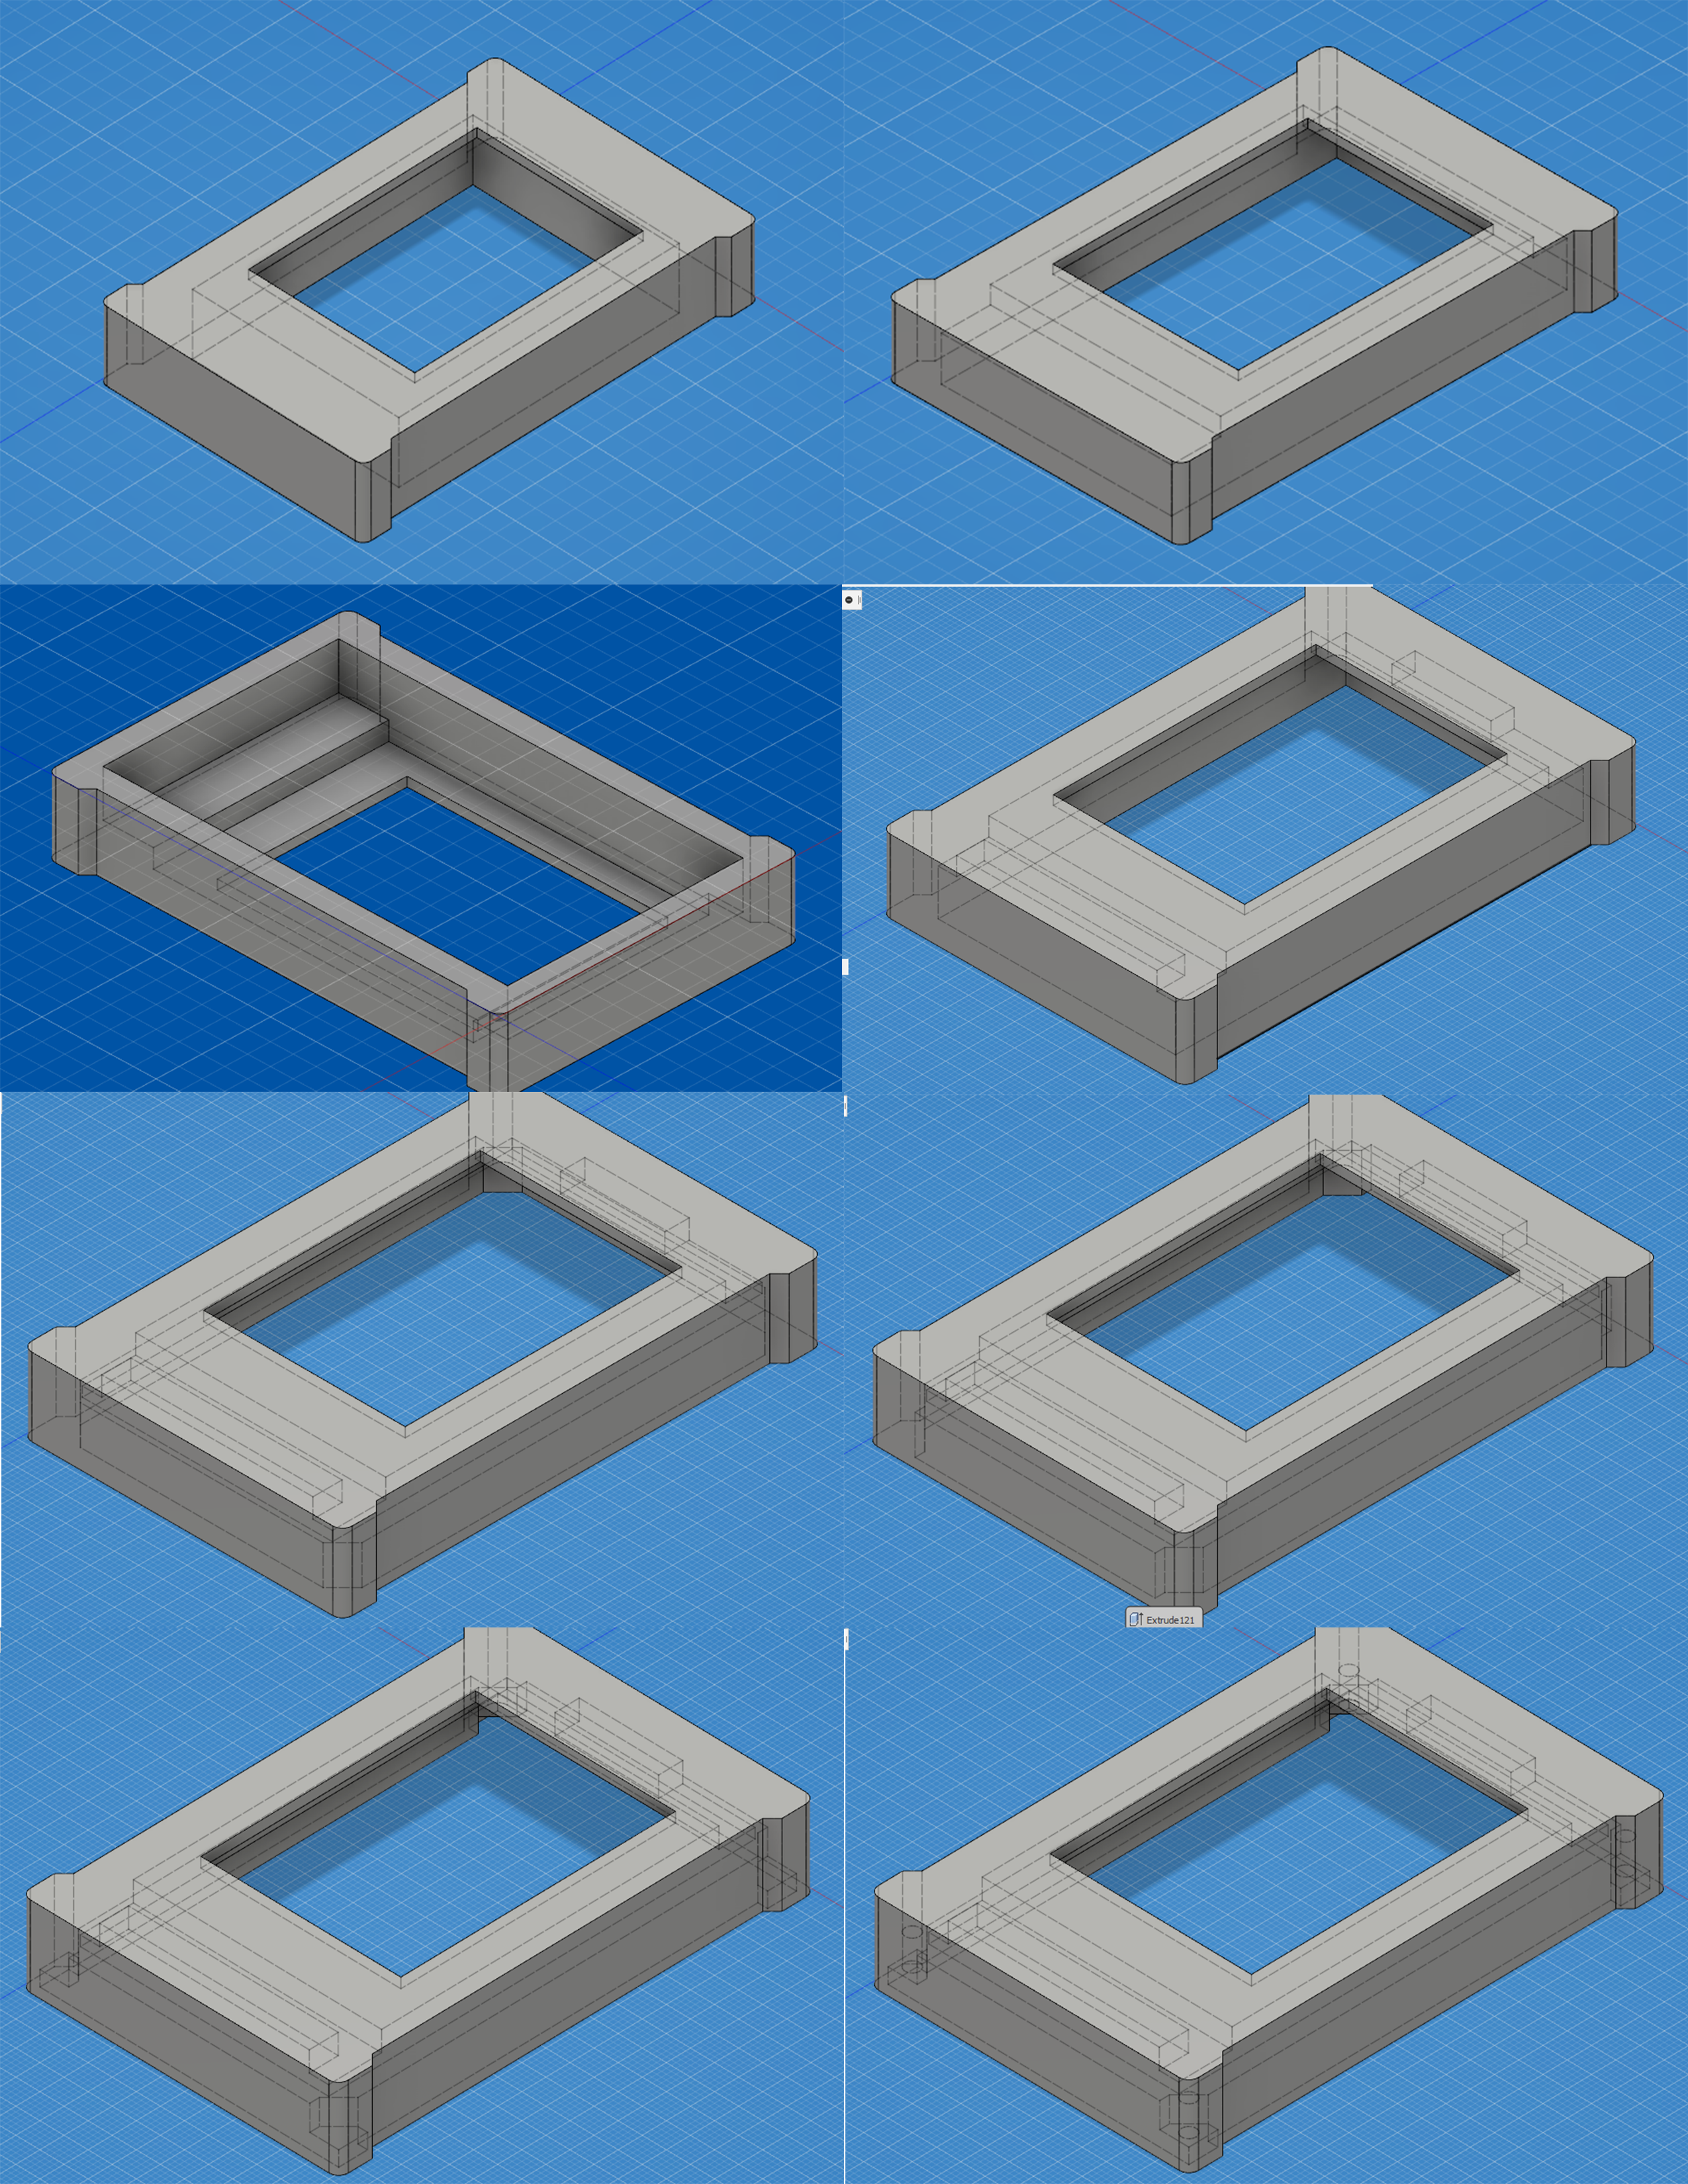
\includegraphics[width=0.8\linewidth]{armazon05.png}
	\caption{Proceso del Diseño del Molde Superior Parte 1}
\end{figure}

\par \noindent
En la figura 4.36 se puede ver como se inicia el diseño del armazón. El diseño del molde superior empieza extrudiendo del dibujo de la figura 4.32; subimos el dibujo unos 17 mm y creamos el orificio donde se vera la pantalla LCD. A partir de allí se empieza a modelar la entrada para la pantalla LCD y el espacio para la placa del prototipo. Una vez diseñado eso en las esquinas se deja un espacio diagonal; específicamente como en la figura 4.34, estos espacios tendrán 3 mm de diferencia con el resto del molde esto es para insertar el molde inferior. Adicional se agregar los orificios donde modelaremos la entrada de tornillos.

\begin{figure}[H]
	\centering
	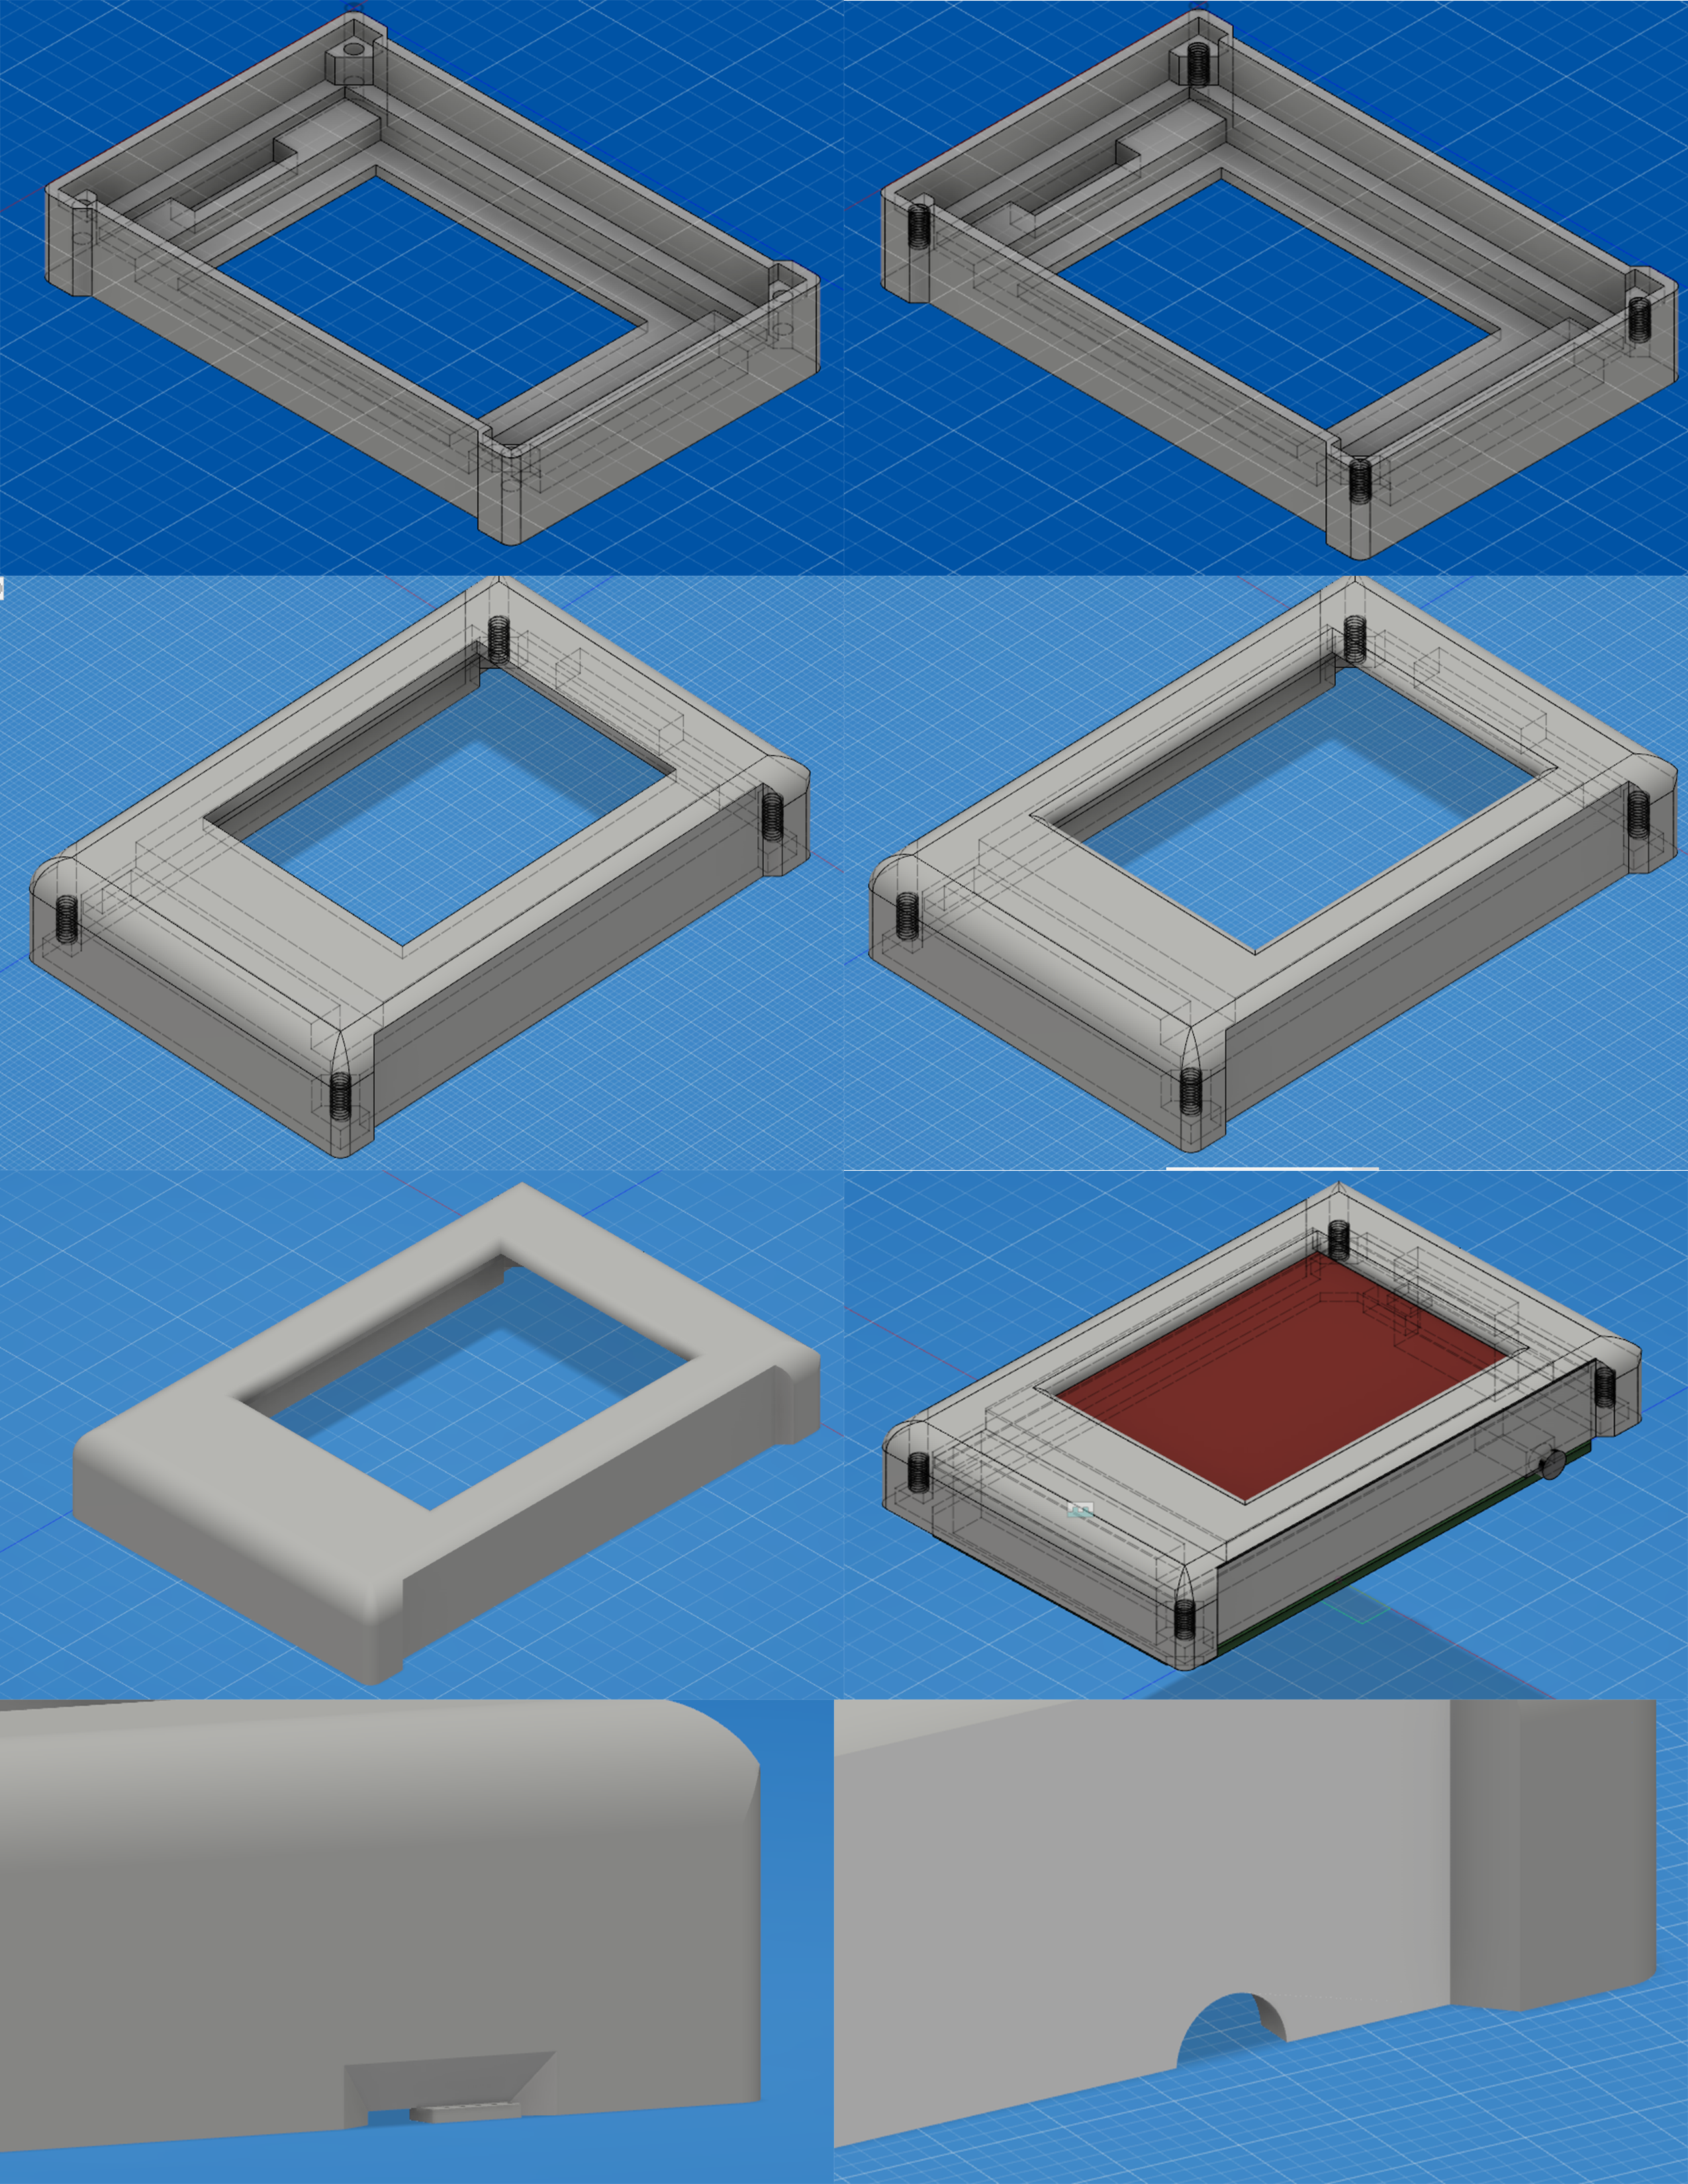
\includegraphics[width=0.8\linewidth]{armazon06.png}
	\caption{Proceso del Diseño del Molde Superior Parte 1}
\end{figure}

\par \noindent
En la figura 4.37 al inicio podemos apreciar todo lo que se realizo en la figura 4.36. Todo esto es para que la pantalla LCD entre sin problemas en el molde. Seguido modelamos las entradas para tornillos en los orificios de las esquinas. Los tornillos para los que estamos modelando son para tornillos de calibre M3. Una vez realizado eso redondeamos los bordes frontales del molde para darle un aspecto mas profesional y por ultimo cortamos los espacios para la entrada del sensor de temperatura y el interruptor para encender el prototipo. El resultado final es el siguiente.

\begin{figure}[H]
	\centering
	\includegraphics[width=0.8\linewidth]{armazon07.png}
	\caption{Diseño del molde superior finalizado}
\end{figure}

\par \noindent
Finalizado el diseño del molde superior procedemos a diseñar el molde inferior.

\subsubsection{Molde Inferior}

\par \noindent
El molde inferior es donde se encontrara la batería de nuestro dispositivo y debe unirse al molde superior y deberá contar con un espacio para que tornillos puedan mantener unido ambos moldes sin problemas. El molde sera basado en los mismos dibujos utilizados por el molde superior. 

\par \noindent
El molde inferior tiene una particularidad y es que debemos tener un espacio para un modulo de carga de la batería por lo que es necesario un corte para la entrada de micro-usb. 

\par \noindent
Observando la imagen 4.38 hay un corte de una circunferencia por donde se conectara el sensor de temperatura. El corte es a la mitad de la circunferencia para una inserción del prototipo al armazón mas sencilla. Adicional hay un espacio en la parte superior del armazón para el interruptor de encendido del prototipo que también se encuentra a la mitad. Ambos cortes debemos tenerlos presentes para el molde inferior. Para mantener la placa sin contacto directo con la batería y tener los cortes necesarios para las entradas del prototipo debemos colocar unos pequeños brazos para que la placa del prototipo tenga donde sostenerse.

\begin{figure}[H]
	\centering
	\includegraphics[width=0.7\linewidth]{armazon08.png}
	\caption{Proceso del diseño del molde inferior parte 1}
\end{figure}

\begin{figure}[H]
	\centering
	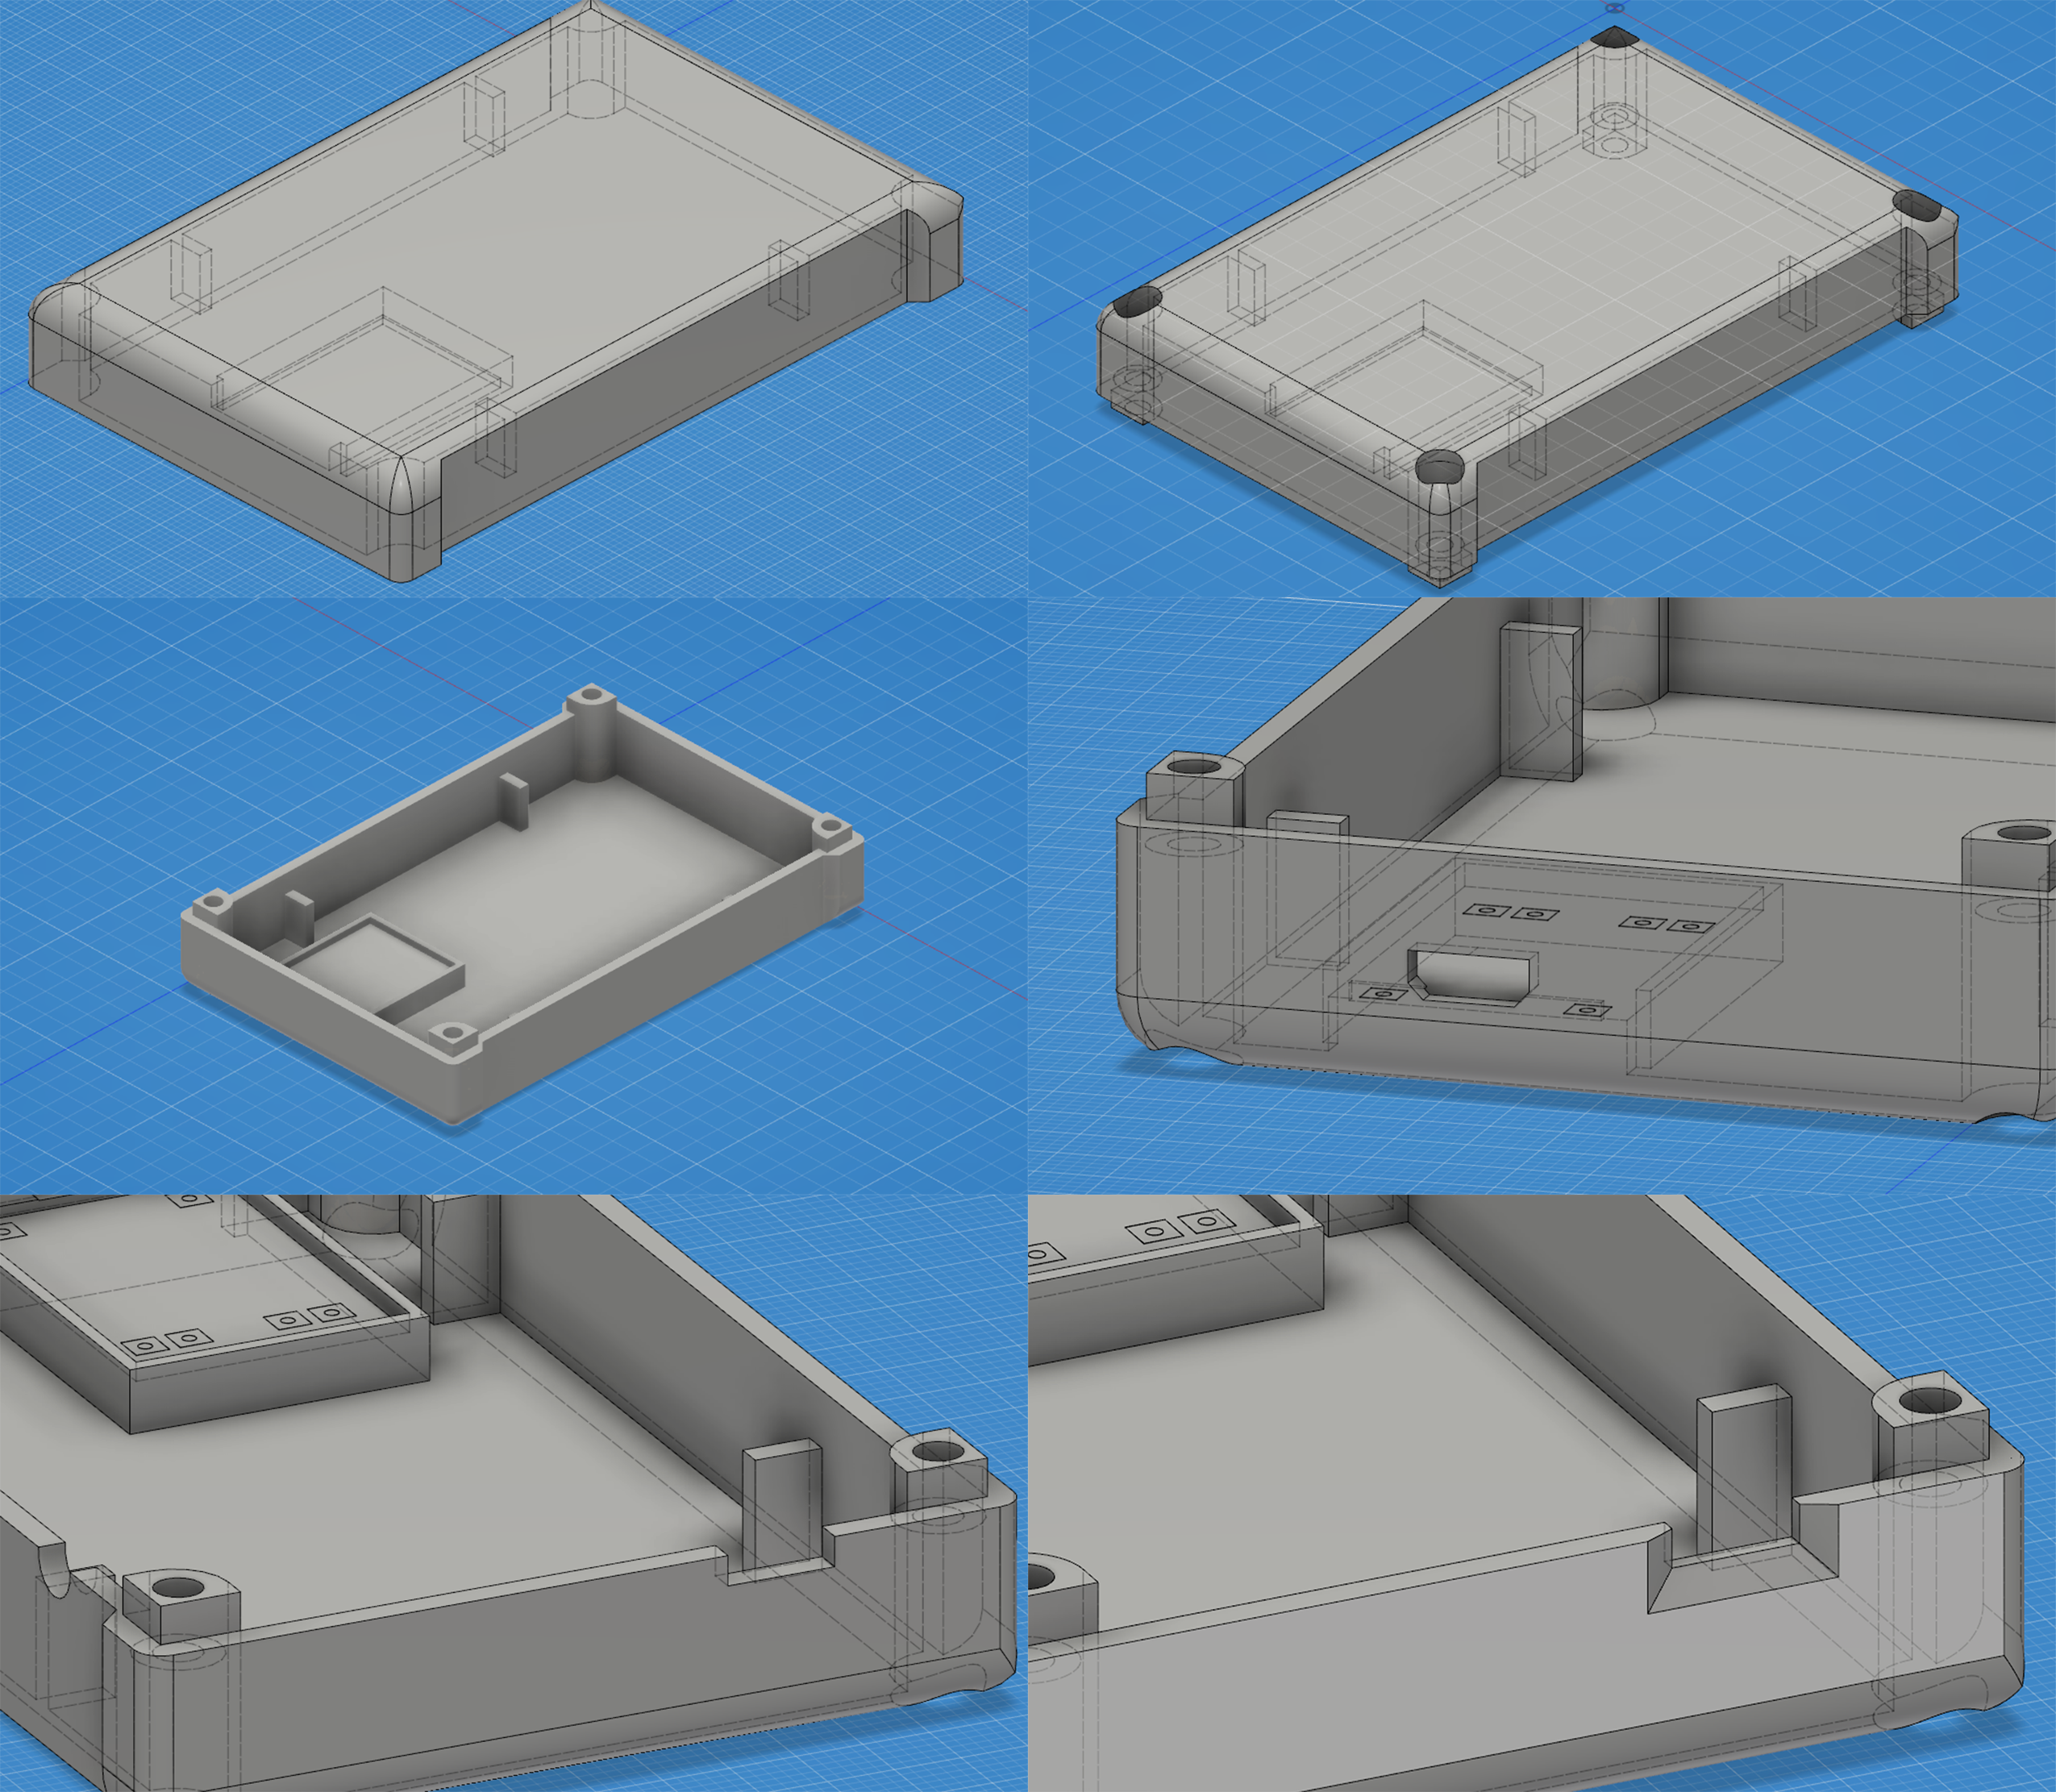
\includegraphics[width=0.7\linewidth]{armazon09.png}
	\caption{Proceso del diseño del molde inferior parte 2}
\end{figure}

\begin{figure}[H]
	\centering
	\includegraphics[width=0.8\linewidth]{armazon10.png}
	\caption{Diseño del molde inferior finalizado}
\end{figure}

\begin{figure}[H]
	\centering
	\includegraphics[width=0.8\linewidth]{armazon11.png}
	\caption{Diseño del final del armazón}
\end{figure}

\par \noindent
Una vez diseñado el molde superior e inferior procedemos a realizar la impresión 3D de los mismos y el ensamblaje final.



\subsection{Ensamblaje Final}

\par \noindent
Para realizar el ensamblaje final del dispositivos debió imprimir los moldes previamente diseñados. La impresora 3D que se utilizó para la impresión del diseño tridimensional es la de la figura 2.22. El resultado de las impresiones son las siguientes:

\begin{figure}[H]
	\centering
	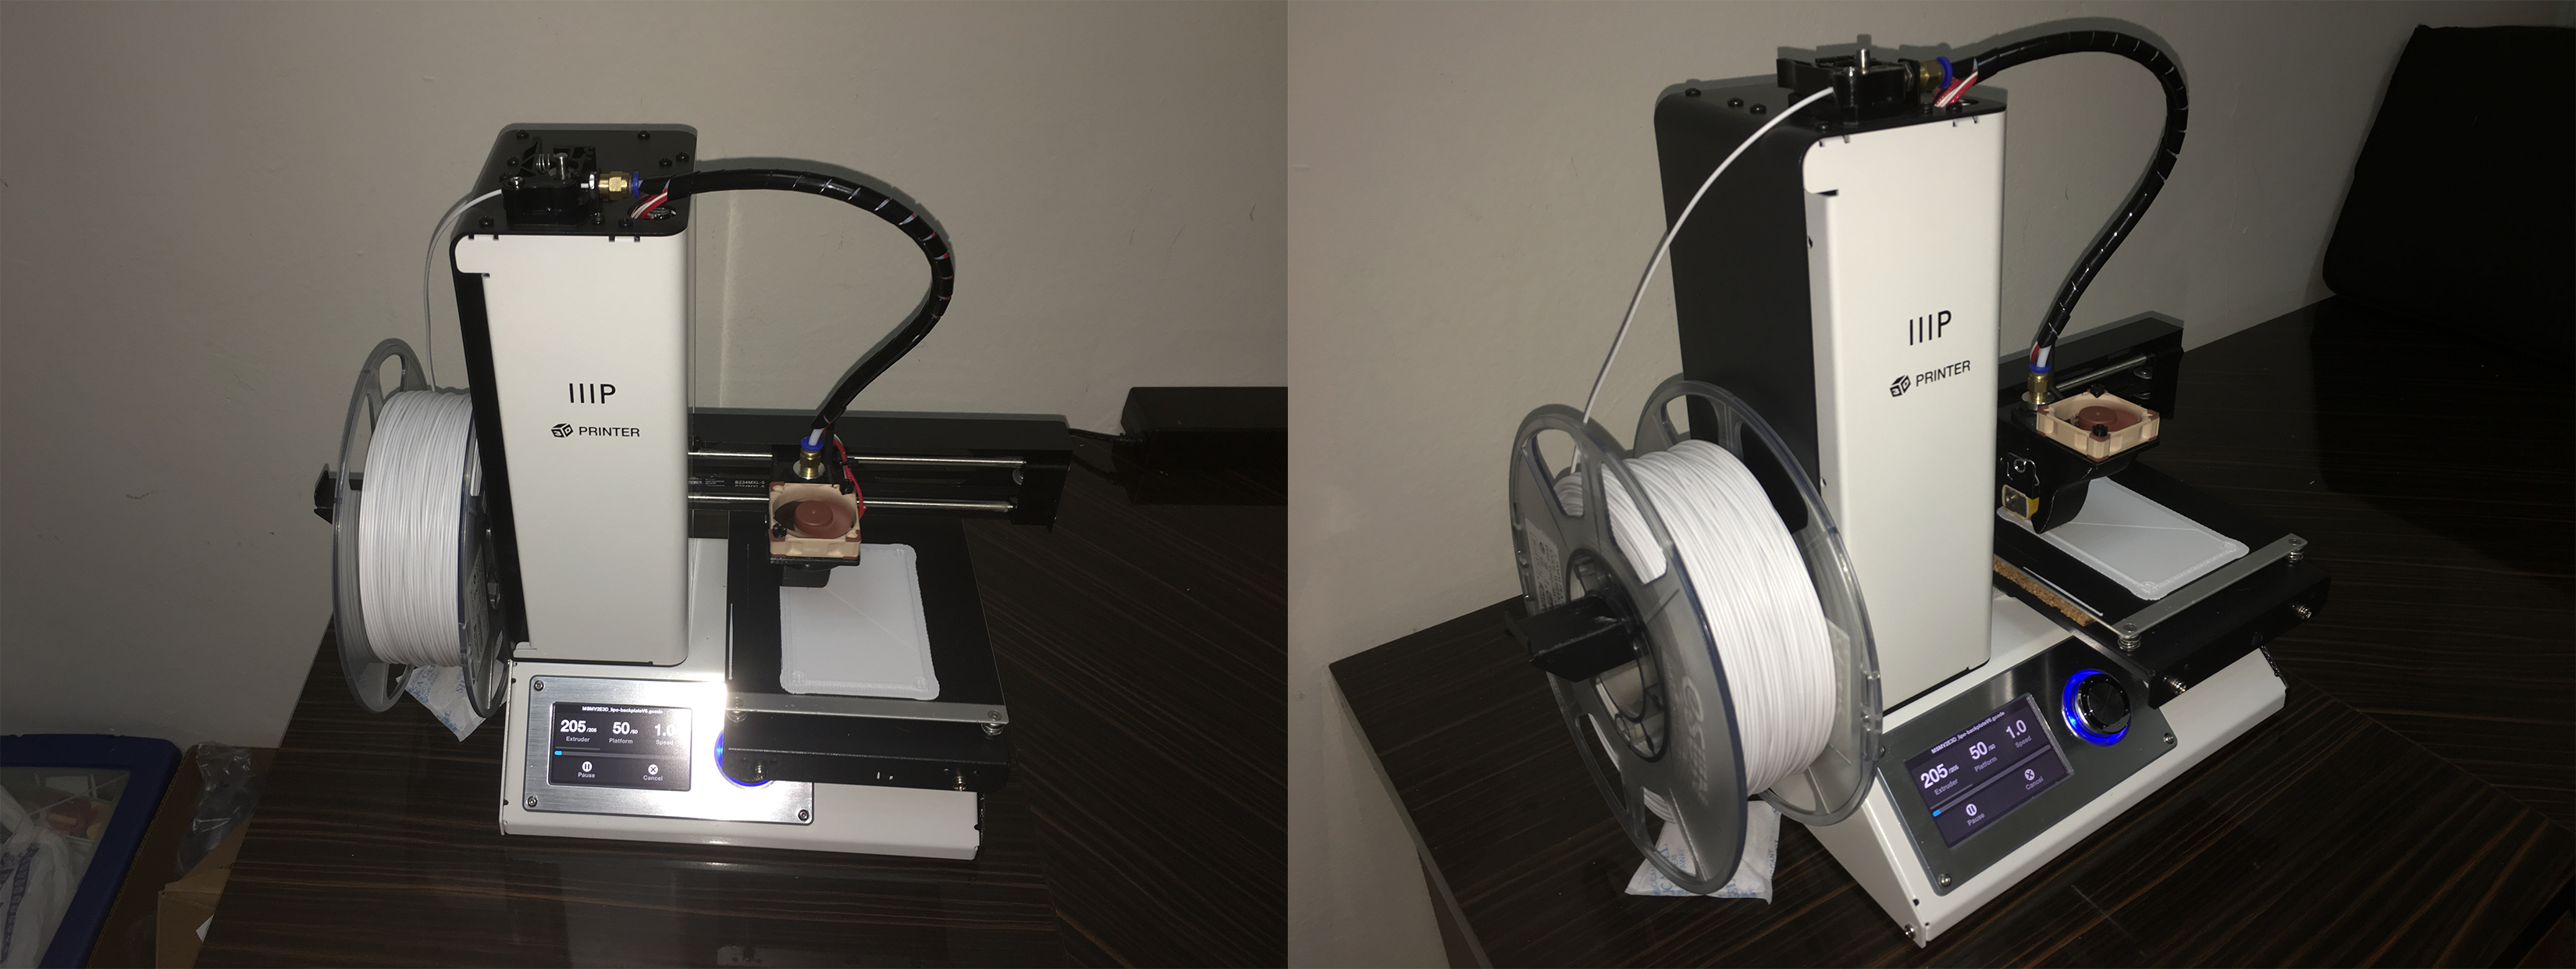
\includegraphics[width=\linewidth]{ensamblaje01.png}
	\caption{Impresora 3D en el proceso de impresión del armazón}
\end{figure}

\begin{figure}[H]
	\centering
	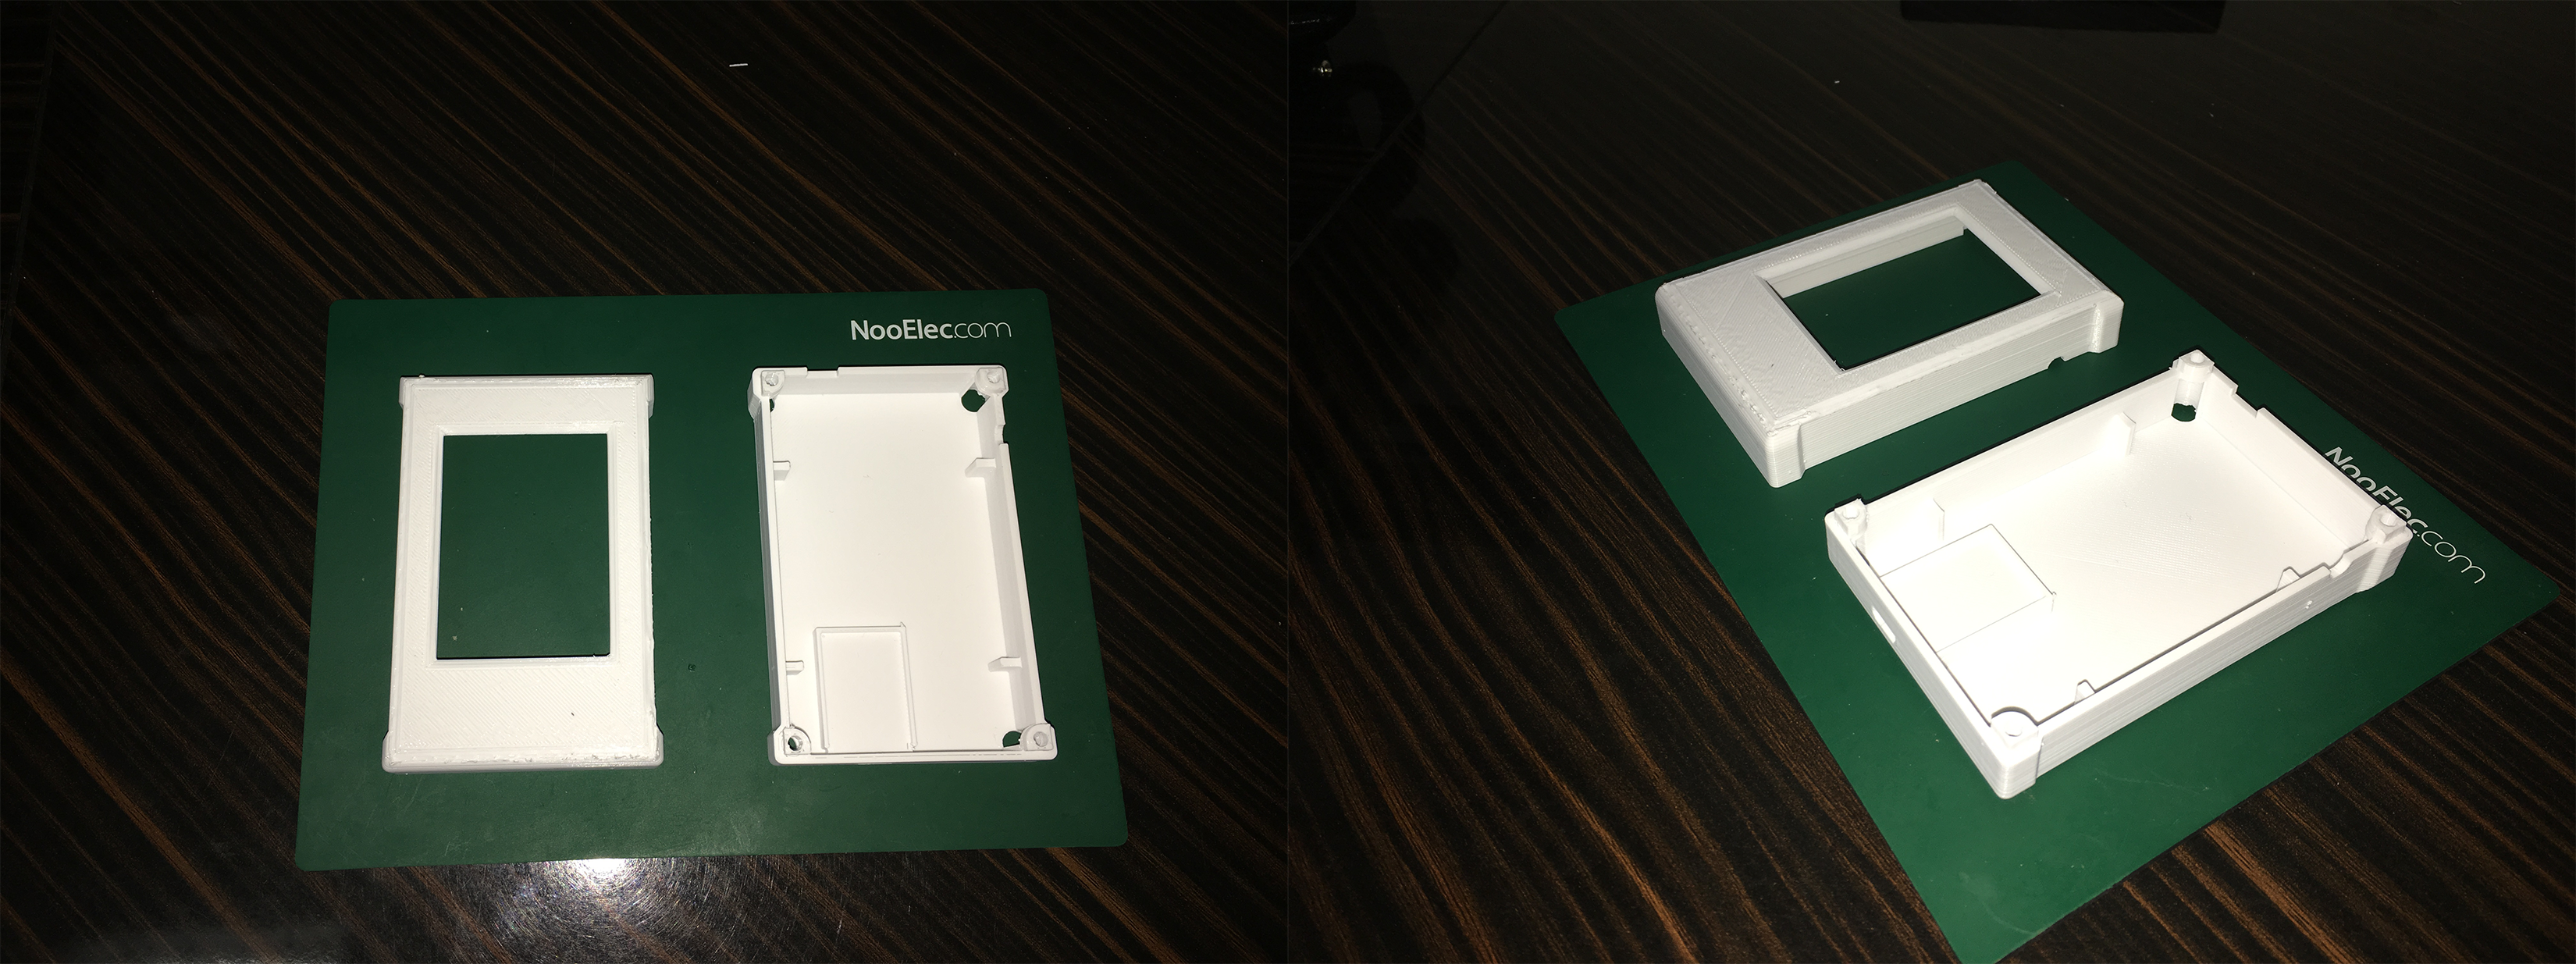
\includegraphics[width=\linewidth]{ensamblaje02.png}
	\caption{Armazón del prototipo hecho por una impresora 3D}
\end{figure}

\par \noindent
El armazón una vez impreso se inicia a soldar los componentes en la placa o circuito impreso del prototipo.

\begin{figure}[H]
	\centering
	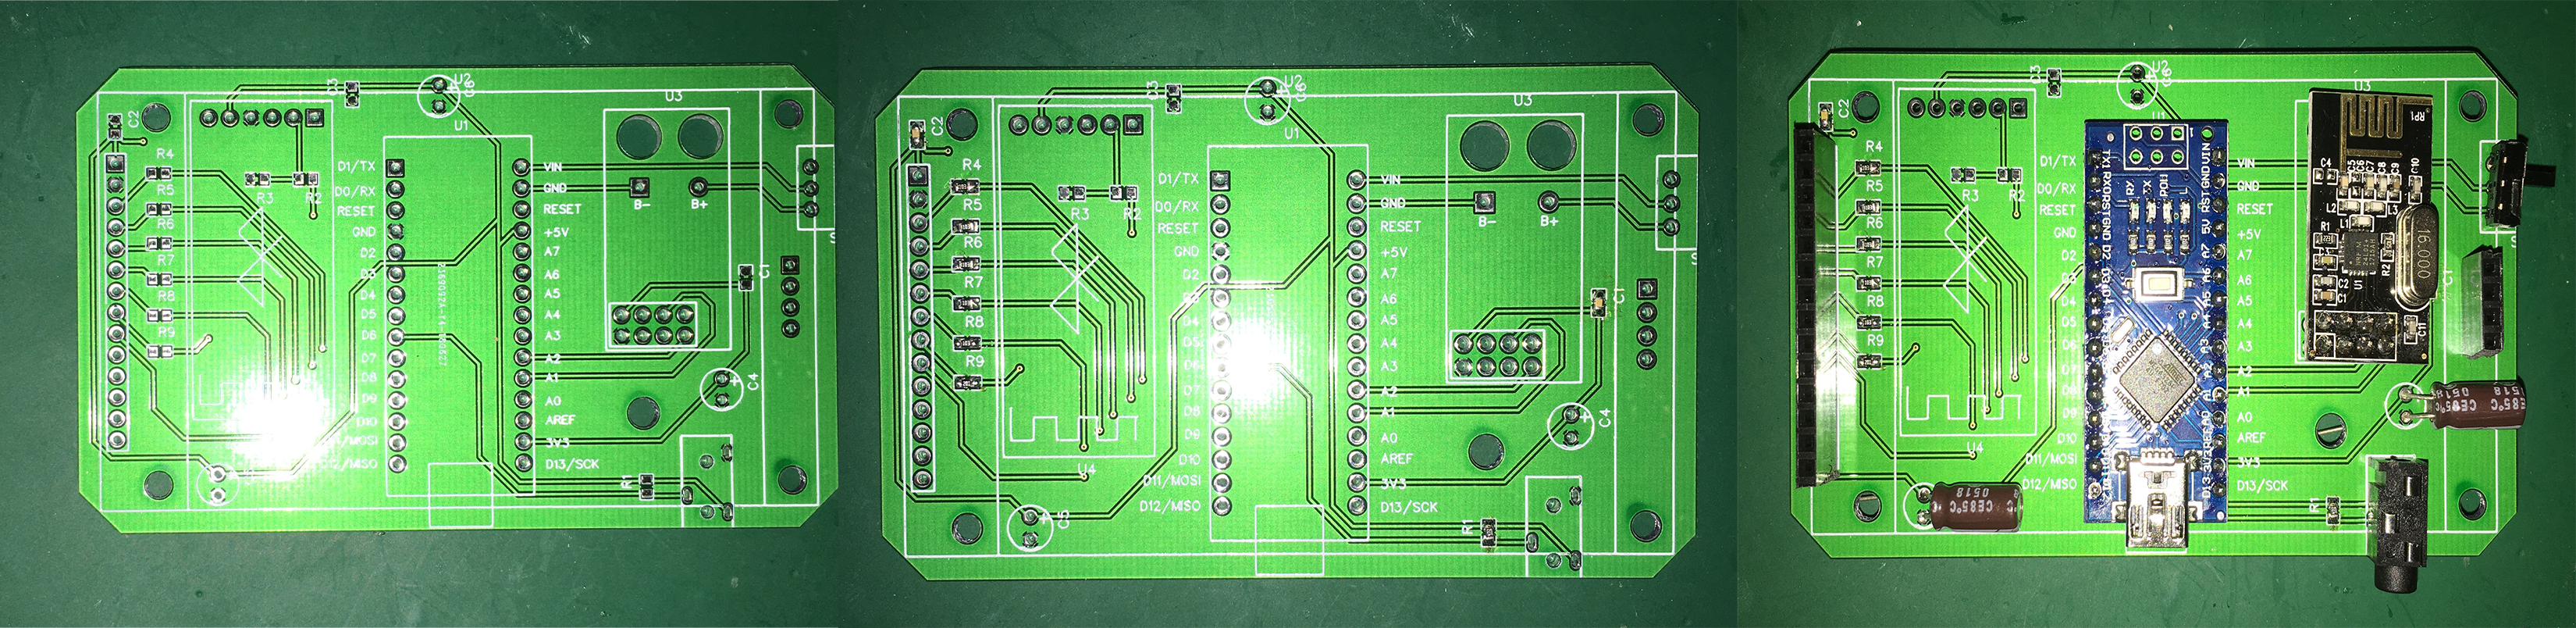
\includegraphics[width=\linewidth]{ensamblaje03.png}
	\caption{Circuito Impreso Antes y Despues de soldar sus componentes}
\end{figure}

\par \noindent
Por ultimo queda colocar la bateria y su circuito en el molde inferior, luego a la placa del dispositivo, después la pantalla LCD y al final colocamos el molde superior.

\begin{figure}[H]
	\centering
	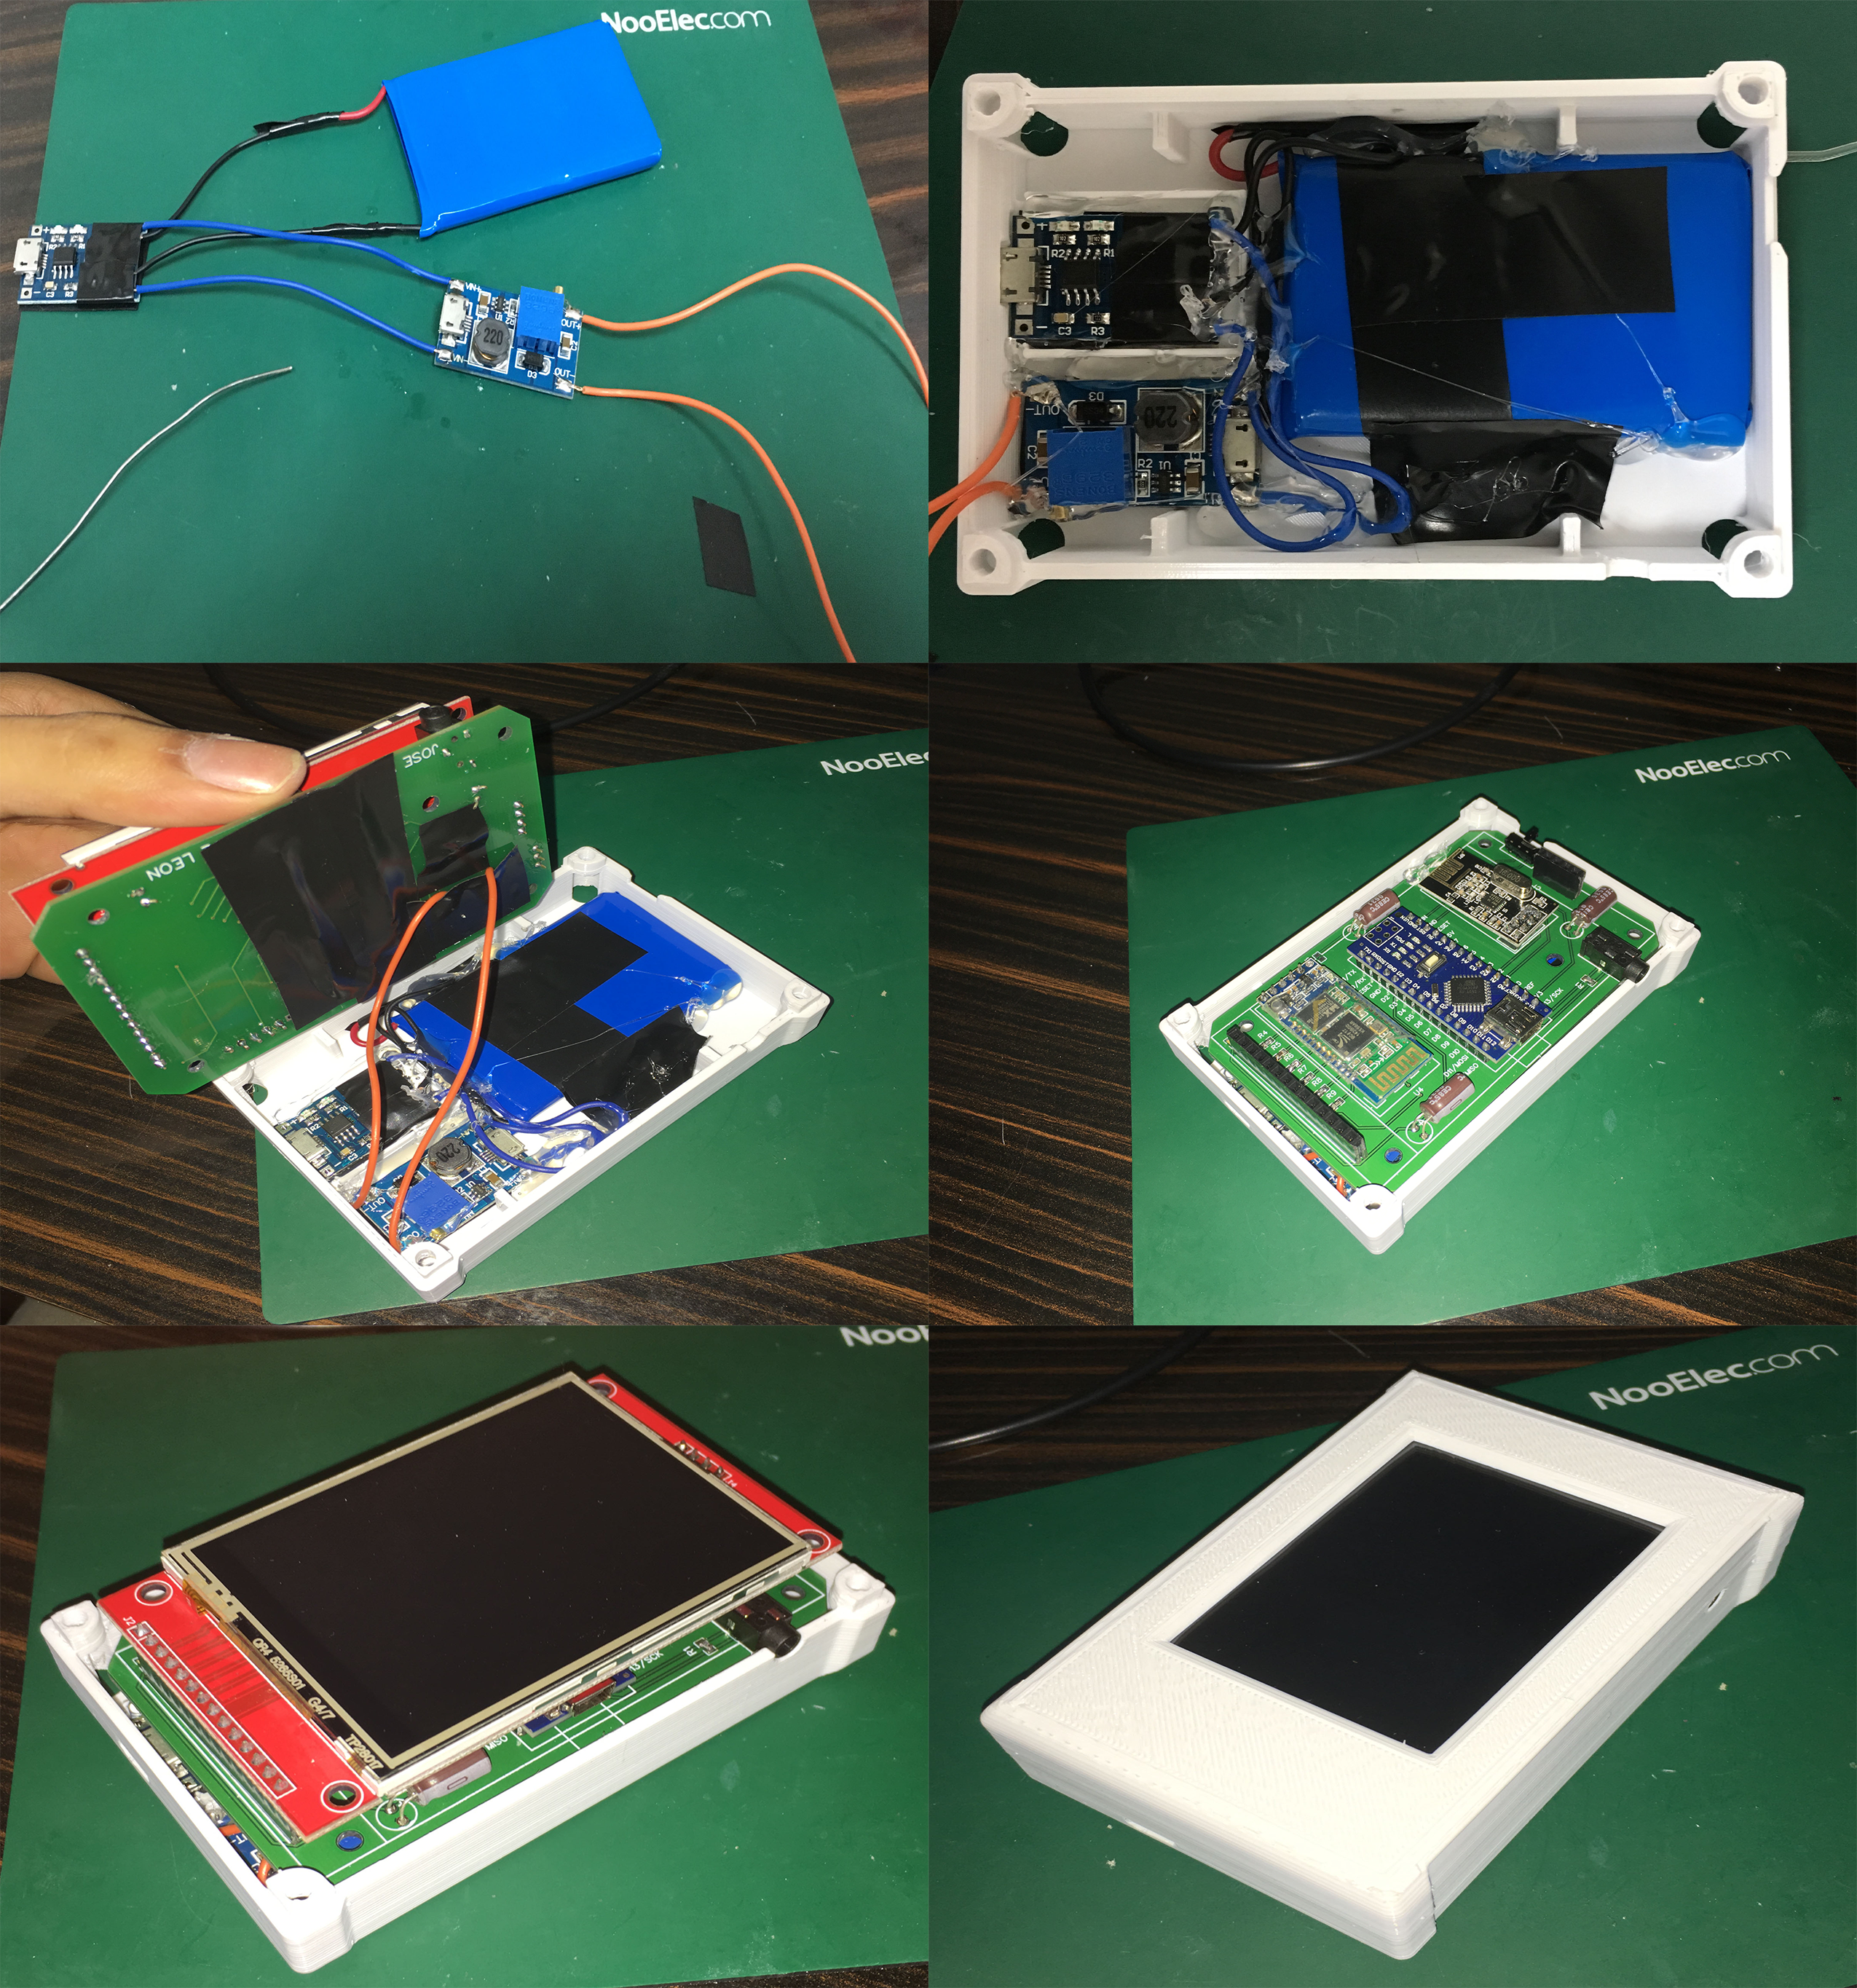
\includegraphics[width=0.8\linewidth]{ensamblaje04.png}
	\caption{Proceso del ensamblaje del prototipo de medición de temperatura}
\end{figure}

\par \noindent
El resultado de unir todas las piezas sería el siguiente:

\begin{figure}[H]
	\centering
	\includegraphics[width=0.8\linewidth]{ensamblaje05.jpg}
	\caption{Prototipo de medición de temperatura completo en su versión 1.0}
\end{figure}

\par \noindent
Ahora que se terminó la elaboración del prototipo deseado, se tomo en cuenta al momento de seleccionar los componentes elegimos el sensor de temperatura DS18B20 por su margen de error y su bajo costo. Ahora la preguntas son las siguientes: ¿El prototipo cumple con los estadares de la compañia SIGCSA? y ¿Cuánto es el costo de la elaboración de un prototipo de estos? para ellos hicierón análisis de las mediciones de temperatura para establecer conclusiones en la sección de resultados.

